\section {Art: The Aesthetic Regime}\label {sec:ArtTheAestheticRegime}

    Jacques Rancière has called the complex system of attitudes, beliefs and behaviours organised by certain ideas about the experience of art the \emph{aesthetic regime}. This regime is not a single coherent paradigm, but a “plurality” of “...frequently different, and sometimes contradictory, ways of thinking...” \citep[p.8]{RanciereMdrnTms2022}. This is a radical repositioning of Aesthetics as art itself, rather than a theory about art.

    \begin{quote}
        [...] Aesthetics [...] denotes neither art theory in general nor a theory that would consign art to its effects on sensibility. Aesthetics refers to a specific regime for identifying and reflecting on the arts: a mode of articulation between ways of doing and making, their corresponding forms of visibility, and possible ways of thinking about their relationships [...] \citep[p.10]{RancierPltcsOfThAsthtcs2004}
    \end{quote}

    The aesthetic regime is superimposed upon, without replacing, the regime of representation \citep[p.50]{RancierPltcsOfThAsthtcs2004}.

    For Rancière, as for others \citep[p.123]{DantoEmbdMnngs2007}, Kant's radical break was to separate sense from sense, by proposing that the essence of an art object lies in its capacity to be experienced without concept. This separation creates a situation in which the effectiveness of an artwork, the very thing that makes it art, is “... a paradoxical kind of efficacy that is produced by the very rupturing of any determinate link between cause and effect.” \citep[p.51]{RancierThEmncptdSpcttr2009}

    \begin{quote}	
        It is precisely this indeterminacy that Kant conceptualized when he defined the beautiful as “what is represented as an object of universal delight apart from any concept”. \citep[p.52]{RancierThEmncptdSpcttr2009}
    \end{quote}	

    Rancière, like Whitehead, Deleuze, Guattari, DeLanda and all the philosophers of process I have been drawing on, is a materialist. \emph{Art} as he has used the term is not a vague generality. Art, synonymous with the aesthetic regime, is a real, individual thing — a ”...determinate historical configuration...” \citep[p.24]{RanciereMdrnTms2022} — that is grounded in the material processes of modern Western life.

    \begin{quote}	
        The cult of art [...] is [...] a recomposition of the landscape of the visible, a recomposition of the relationship between doing, making, being, seeing, and saying. Whatever might be the specific type of economic circuits they lie within, artistic practices are not “exceptions” to other practices. They represent and reconfigure the distribution of these activities. \citep[p.45]{RancierPltcsOfThAsthtcs2004}
    \end{quote}	
    
    For Rancière, the emergence of the aesthetic regime of art is a collective political act, a tactic for resisting social stratification and capitalist equations involving labour, production and value by carving out a space for the sensible that is not reducible to the intelligible. It is a kind of democratising hack for a sociopolitical situation in which taste and judgement were tightly coupled with social status. Along with Kant, Rancière rates as \emph{unsurpassable}, Schiller's \emph{On the Aesthetic Education of Man: and, Letters to Prince Frederick Christian von Augustenburg} which was published soon after Kant's \emph{Critique} (1794), and which he describes as “[...] this regimes first manifesto” \citep[pp.23-24]{RancierPltcsOfThAsthtcs2004}.
        
    
    \begin{quote}	
        Schiller's “aesthetic” state, by suspending the opposition between active understanding and passive sensibility, aims at breaking down - with an idea of art - an idea of society based on the opposition between those who think and decide and those who are doomed to material tasks. \citep[p.44]{RancierPltcsOfThAsthtcs2004}
    \end{quote}	

    The manoeuvre of asserting the autonomy of an art based solely on aesthetic experience, of carving off a space for the sensible that is not reducible to pre-existing concepts, and which must be connected to other aspects of life only indirectly and indeterminately\postnote{

        The separation from other aspects of culture, a key characteristic Western art in general, is not a universal characteristic of art across cultures. Artmaking plays a different, more integrated, role in Indigenous Australian cultures, for example \citep{MorphyTMnyMngs1977}. Heidegger, in his essay \emph{The Question Concerning Technology}, suggested that for the the ancient Greeks the practices we now call \emph{craft} and the \emph{fine arts} were not separate but were part of a single class of practices called \emph{technē}, along with the practices we now call philosophy and science.

        \begin{quote}
            We must observe two things with respect to the meaning of this word. One is that \emph{technē} is the name not only for the activities and skills of the craftsman, but also for the arts of the mind and the fine arts. \emph{Technē} belongs to bringing-forth, to \emph{poiesis}; it is something poietic. \citep[pp. 12,13]{HeideggerThQstnCncrngTchnlgy1954}
        \end{quote}

        If Heidegger is right, then clearly a lot has happened to get us from \emph{technē} to the current state where Contemporary art exists as a distinct style within a tradition of \emph{fine art}, which is different from craft, philosophy and science — all of which have a myriad of subcategories. Complexity scientists and process philosophers would certainly describe this process of progressive differentiation as a \emph{symmetry breaking cascade}\postnote{DeLanda quote perhaps}.

    }, creates a regime in which anything can, potentially, be art: “Art exists as a separate world since anything whatsoever can belong to it.” \citep[p.X]{RancièreAisthesis2013} 

    \begin{quote}	
        The aesthetic regime of the arts is the regime that strictly identifies art in the singular and frees it from any specific rule, from any hierarchy of the arts, subject matter, and genres. Yet it does so by destroying the mimetic barrier that distinguished ways of doing and making affiliated with art from other ways of doing and making [...] The aesthetic regime asserts the absolute singularity of art and, at the same time, destroys any pragmatic criterion for isolating this singularity. It simultaneously establishes the autonomy of art and the identity of its forms with the forms that life uses to shape itself. \citep[p.23]{RancierPltcsOfThAsthtcs2004}
    \end{quote}	

    One of the key features of the aesthetic regime, according to Rancière, is the way it enables objects created under other regimes — for purposes other than aesthetic appreciation — to be experienced as art. A kind of transfiguration, or dislocation, occurs when an object is brought into the aesthetic regime. The object is no longer understood in terms of its original function or purpose, but as an object of contemplation within the aesthetic regime.

    \begin{quote}
        The works that entered the realm of aesthetic experience at the time when museums were created had originally been produced for a particular destination: the civic festivals of antiquity, religious ceremonies, the decorum of monarchic power or aristocratic life. But the aesthetic regime separated them from those functions and destinations. The aesthetic sensorium is the sensorium marked by that loss of destination. What is lost, along with the harmony between poiesis and aisthesis, is the dependence of artistic productions on a distribution of social places and functions. The previous destination of works corresponded to a certain order of bodies, a certain harmony between the places and functions of a social order and the capacities or incapacities of the bodies located in this or that place, devoted to this or that function. \citep[p.56]{RancierThEmncptdSpcttr2009}
    \end{quote}

    It is not simply that objects \emph{can} be transfigured into art objects, but that the aesthetic regime \emph{is} a system of codes that dislocates objects from their original functions and meanings. For Rancière, the aesthetic experience is therefore a kind of \emph{dissensuality}\postnote{

        \begin{quote}
            The dissensual operation takes the form of a superimposition that transforms a given form or body into a new one. \citep[p.54]{RancierThEmncptdSpcttr2009}
        \end{quote}

    }.
    
    For Rancière, this process is not entirely synonymous with the “...Deleuzian dramaturgy...” of art as a bloc of pure sensation, which is for him “...too indebted to the modernist dramaturgy of the sublime break. It obscures the form of dissensuality that is specific to aesthetic work...” \citep[p.54]{RancierThEmncptdSpcttr2009}.
        
    \subsection{Aesthetic Experience as Affect}\label{sec:AestheticExperienceAsAffect}

        For theorists who used the term \emph{affect} and who also write about art, affect is synonymous with aesthetic experience. For example, Guattari used the terms interchangeably when talking about art objects:

        \begin{quote}
            One gets to know them not through representation but through affective contamination. They start to exist in you, in spite of you. And not only as crude, undifferentiated affects, but as hyper-complex compositions [...] The paradox which aesthetic experience constantly returns us to is that these affects, as a mode of existential apprehension, are given all at once, regardless, or besides the fact that indicative traits and descriptive refrains are necessary for catalysing their existence in fields of representation. \citep[pp. 92-93]{GuattariChsmss1995}
        \end{quote}

        This is arguably a kind of return to a pre-Kantian aesthetics \citep[p.121]{HighmoreBttrAftrTst2010}. The field of Aesthetics had been developing for 40 years or so before Kant's \emph{Critique of Judgement} was published in 1790. Contemporary scholars attribute its inception to the work of European philosophers Christian Wolff and his disciples, including Moses Mendelssohn and, especially, Alexander Baumgarten \citep[pp.327-338]{EagletonFrPrtclrs1990}. Baumgarten thought that the Cartesian philosophical emphasis on logic and conceptual thought had neglected the epistemological role of sensorial experience. For Baumgarten, aesthetic cognition mediated between reason and sense; the aesthetic was a kind of (inferior, feminine) analogue of reason, operating at the level of material life. Within the dense amorphous flow of our sensuous experience, constantly in flux, certain objects stand out in a kind of ideality akin to rational perfection, which is beauty. \citep[p.328]{EagletonFrPrtclrs1990}. Kant's \emph{Critique} was a distillation of aesthetic experience down to two categories: the beautiful and the sublime\postnote{

            This process was probably already happening before Kant wrote his \emph{Critique}. In it, he referred to a 1757 treatise on aesthetics written by Edmund Burke called \emph{A Philosophical Enquiry into the Origin of Our Ideas of the Sublime and Beautiful}. 

        }.
        
        Kant's \emph{Critique} also formalised the connection between aesthetic experience and art. Through various universalising appeals to ideas of morality and common sense, he positioned the beautiful as that which is experienced as being pleasing by being \emph{purposive without purpose}, and this is exemplified by our experience of art. The sublime is 
        that which is experienced as a kind of rapid toggling back and forth between fear and pleasure in response to an awe-inspiring natural subject \postnote{

            “The feeling of the sublime is [...] at once a feeling of displeasure, arising from the inadequacy of imagination in the aesthetic estimation of magnitude to attain to its estimation by reason, and a simultaneously awakened pleasure, arising from this very judgement of the inadequacy of the greatest faculty of sense being in accord with ideas of reason, so far as the effort to attain to these is for us a law [...] The mind feels itself set in motion in the representation of the sublime in nature [...] This movement, especially in its inception, may be compared with a shaking, i.e. with a rapidly alternating repulsion and attraction produced by one and the same object.“ \citep[p.88]{KantCrtqOfJdgmnt}

        }. From a perspective informed by complexity thinking and process philosophy, this narrowing down of the officially sanctioned range for aesthetic experience, and its becoming welded to the idea of art, seems absurd. Highmore asked, with some exasperation:

        \begin{quote}
            [...] how does a form of inquiry that was once aimed at the entire creaturely world end up as a specialized discourse about fine art? How did an ambitious curiosity about the affects, the body, and the senses end up fixated on only one tiny area of sensual life — beauty and the sublime? [...] \citep[p.121-122]{HighmoreBttrAftrTst2010}
        \end{quote}

        While many people are content to blame Kant, he suggests that the answer was present in aesthetic discourse from the start and that it takes two forms. 

        \begin{quote}
            First is the a priori assumption that certain experiences are simply better than others thus beauty will win out over boredom each and every time because beauty is seen as edifying and morally uplifting whereas boredom would simply register as the failure of self-discipline and moral vigilance ("the devil makes work for idle hands"). Second is the difficulty of speaking and writing about creaturely, experiential life, except through exemplification (an exemplification that is most often provided by art). It is this second characteristic of aesthetic discourse that results in the misdirection of aesthetics, directing it to become simply synonymous with art theory [...] Here the artwork is a moral lesson, an aesthetic example to be mimicked and developed for the pursuit of the good and the true.\citep[p.122]{HighmoreBttrAftrTst2010}
        \end{quote}

        Danto was one of the first to point out the absurdity of the idea that aesthetic experiences are synonymous with the experiences of beauty (sublimity hardly gets a mention by Danto). It is arguably a kind of philosophical colonialism \citep[p.124]{DantoEmbdMnngs2007}, since it requires a subjective, culturally informed, experience to function as an objective definition. It sets acceptance of a normative idea as the price of admittance into the world of art. Clearly, the work of many Contemporary artists simply doesn't make sense along side such a restrictive definition of aesthetic experience. A focus on beauty has had the effect of delegitimising the real diversity of aesthetic experiences available to artists \citep[p.59]{DantoThAbsOfBty2003}, which might be based in virtually any kind of observed quality, like cuteness \citep[p.28]{DantoThPhlsphclArt2005}, grunge, blandness \citep[p.126]{DantoEmbdMnngs2007}, disgustingness, eroticism, \citep[p.59]{DantoThAbsOfBty2003}, et cetera.

        \begin{quote}
            [...] there is scarcely a predicate of ordinary discourse which cannot be pressed into aesthetic service. So there are fluid drawings and clunky drawings, fragile drawings and witty drawings, explosive drawings and childlike drawings of flowers which even in the most likely case are probably not fragile by anything like the same criteria drawings of them are. \citep[pp. 28-29]{DantoThPhlsphclArt2005}
        \end{quote}

        The move to equate aesthetic experience with affect is a shift away from the idea that some experiences are better than others and the artwork is a moral lesson, and towards the messy reality of the ongoingness of process. It contextualises aesthetic experience in a complex ecology of affects, intensities, and sensations. As Highmore put it, referencing Guattari:

        \begin{quote}
            [...] there are complex affective and intensive exchanges, situated in the broader ecology of the world. \citep[p.155]{HighmoreBttrAftrTst2010}
        \end{quote}

        Art is no longer about representation.

		\begin{quote}
		    [...] a block of percept and affect, by way of aesthetic composition, agglomerates in the same transversal flash the subject and object, the self and other, the material and incorporeal, the before and after .... In short, affect is not a question of representation and discursivity, but of existence. I find myself transported into a Debussyst Universe, a blues Universe, a blazing becoming of Provence. I have crossed a threshold of consistency. Before the hold of this block of sensation, this nucleus of partial subjectivation, everything was dull, beyond it, I am no longer as I was before, I am swept away by a becoming other, carried beyond my familiar existential Territories.
		\citep[p.93]{GuattariChsmss1995}
		\end{quote}

    \subsection{Blocs of Sensation, Affective Assemblages}\label{sec:BlocsOfSensationEntropyMachines}

        In \emph{What Is Philosophy} Deleuze and Guattari describe the nature of artmaking as a process of aesthetic \emph{composition} that results in the creation of a \emph{compound of sensation}.

        \begin{quote}
            There is only a single plane in the sense that art includes no other plane than that of aesthetic composition [...] It is on this condition that matter becomes expressive: either the compound of sensations is realized in the material, or the material passes into the compound, but always in such a way as to be situated on a specifically aesthetic plane of composition. There are indeed technical problems in art [...] but they are posed only as a function of aesthetic problems of composition that concern compounds of sensation and the plane to which they and their materials are necessarily linked. Every sensation is a question, even if the only answer is silence. In art the problem is always that of finding what monument to erect on this plane, or what plane to slide under this monument, and both at the same time [...] \citep[pp. 195-196]{DeleuzeGuattariWhatIsPhilosophy1994}
        \end{quote}

        An art object, this \emph{compound}, is also referred to as a \emph{bloc of sensation}:

        \begin{quote}
            What is preserved — the thing or the work of art — is a bloc of sensations, that is to say, a compound of percepts and affects. \citep[p.164]{DeleuzeGuattariWhatIsPhilosophy1994}
        \end{quote}

        An artwork is a \emph{bloc} because its properties and capacities cannot be reduced to the properties and capacities of the materials from which it is made. They are emergent. Like pretty much everything when viewed from the right angle, an artwork is an \emph{assemblage} — a complex system. Zepke has called art objects \emph{affectual assemblages} \citep[p.6]{ZepkeArtAsAbstrctMchn2005}.


        % \begin{quote}
        %     When information enters the domain of life, it becomes vital dynamism. \citep[p.236]{ZepkeOSullivanDlzCntmprryArt2010}
        % \end{quote}

        % \begin{quote}
        %     [...] information acquired by perceptual and sensational states is transduced into emotional and affective life. This process leads to an operation of individuation that positions the subject within the world \citep[p.236]{ZepkeOSullivanDlzCntmprryArt2010}
        % \end{quote}

    \subsection{Probe Heads} \label{sec:ProbeHeads}
        
        For Deleuze and Guattari, and for the scholars and artists who have been inspired by concepts like \emph{line of flight}, \emph{refrain}, and \emph{machine}, artmaking is a way of going beyond the constraints of the present by generating new realities \citep[p.3]{ZepkeOSullivanDlzCntmprryArt2010}. Art objects are \emph{probe heads} “...that dismantle the strata [...], break through the walls of signifiance, pour out of the holes of subjectivity, fell trees in favor of [...] rhizomes, and steer the flows down lines of positive deterritorializaton or creative flight” \citep[p.190]{DeleuzeGuattariAThousandPlateaus1987}. They are the leading edge of a process of sociocultural exploration and creation.

        Artists, it is proposed, don't just create art objects, but new contexts — new realities — within which the these objects have meaning and affective power. Art is a way of worlding the world, of probing and going beyond current limits of possibility.

        \begin{quote}
            [...] artistic practice has both an impact in the domain of the sensitive, in the domain of percepts and affects, and at the same time a direct influence on the production of universes of values, of universes of reference and centers of subjectivation. \citep[p.4]{GuattariOlivierFlxGttrEtLArtCntmprn1994}\postnote{

                This is a machine translation of the original French, which is:

                \begin{quote}
                    [...] la pratique artistique a à la fois un impact dans le domaine du sensible, dans le domaine des percepts et des affects, et en même temps une prise directe sur la production d”univers de valeurs, d”univers de référence et de foyers de subjectivation. \citep[p.4]{GuattariOlivierFlxGttrEtLArtCntmprn1994}
                \end{quote}
            }
        \end{quote}

        Artists makes art objects, but the actual change takes place in and through the affective experiences that are generated when these objects are received.

        \begin{quote}
            When I "consume" a work [...] I carry out a complex ontological crystallisation, an alterification of beings-there. I summon being to exist differently and I extort new intensities from it [...] \citep[p.96]{GuattariChsmss1995}
        \end{quote}

        Guattari used the invention of polyphonic music as an example of how art creates new realities:

		\begin{quote}
    		[...] We can no longer act as though polyphonic music had not been invented for the rest of time, both past and future. \citep[pp. 27-28]{GuattariChsmss1995}
		\end{quote}

        New realities are not meant to be easy, and this kind of art is not made to be comforting. It is designed to change us. It is a calling into existence of a new kind of human. Art, says Simon O'Sullivan is “...ontologically difficult...”. It “...calls its audience into being.” It “...summons forth [...] new people” \citep[p.68]{OSullivanArtEncntrs2006}.
        
        Artists, according to this way of thinking, have responsibilities. This process of creating new realities and summoning into existence new people has ethical, even political implications.

		\begin{quote}
		    [...] The new aesthetic paradigm has ethico-political implications because to speak of creation is to speak of the responsibility of the creative instance with regard to the thing created, inflection of the state of things, bifurcation beyond pre-established schemas [...] \citep[p.107]{GuattariChsmss1995}
		\end{quote}

        Stephen Zepke has traced this ethical imperative back through Deleuze and Guattari to Nietzsche and Spinoza. Nietzsche thought that the values of his time were nihilistic, and that art has the capacity to be life-affirming.

        \begin{quote}
            Art [...] is first of all a process of self-creation, an ethical and ontological practice as much as on aesthetic one. This, Nietzsche claims, is a “Higher concept of art” that no longer simply describes an object, nor a subjective process, but a mechanism by which the creativity of life, the “will to power” as Nietzsche called it, is expressed in life. \citep[p.12]{ZepkeArtAsAbstrctMchn2005}
        \end{quote}

        As an example, Zepke referred to Deleuze's affirmation of Andy Warhol's work, and of Pop Art's strategy of repetition in general. 

        \begin{quote}
            The Warhol-machine understood perfectly that the work of art had lost its aura as original in the age of mechanical reproduction. But he refused to mourn this loss, and instead embraced the living power of repetition it introduces [...] Warhol is the artist of the little difference, but his affirmation of mechanical repetitions nevertheless produced a new relation between art and the world. \citep[p.35-36]{ZepkeArtAsAbstrctMchn2005}
        \end{quote}

        Spinoza, Zepke suggested, provided Deleuze with a mystical dimension, an atheism in which God is nature, “...the infinite unfolding of what expresses itself, the explication of the One in the many” \citep[p.42]{ZepkeArtAsAbstrctMchn2005}. In this context,

        \begin{quote}
            [...] an ethical-aesthetic will affirm joyful affects in constructing a new mode of existence, an existence that expresses God, and understands this expression as a becoming through which God constructs and so understands itself. This will be the atheistic mysticism of art. \citep[p.52]{ZepkeArtAsAbstrctMchn2005}
        \end{quote}

        Ironically, the method of creating new realities involves working with falsehoods. In a reality in which everything is process, in which there is no being only always becoming, there is no such thing as truth.
        Aesthetics, Zepke has reminded us, “...cannot be a science of representation, because quite simply there is nothing to represent. Art without truth; it means that art is nothing but the creation of falsehood.” \citep[p.19]{ZepkeArtAsAbstrctMchn2005}. He quotes Deleuze repeating Nietzsche:
        
        \begin{quote}
            The world is neither true nor real but living. And the living world is will to power, will to falsehood, which is actualised in many different powers. To actualise the will to falsehood under any quality whatever, is always to evaluate. To live is to evaluate. There is no truth of the world as it is thought, no reality of the sensible world, all is evaluation, even and above all the sensible and the real. (NI 184/191—2) \citep[p.19]{ZepkeArtAsAbstrctMchn2005}
        \end{quote}

        In the aesthetic regime, the artist doesn't represent or communicate truth, but composes blocs of sensation that are complex enough to meet the complexity of the world.

        \begin{quote}
            Who speaks the truth? This is no longer the question; but how, and under what conditions can the best bring about the pragmatics of incorporeal events that will recompose a world and reinstall processual complexity? \citep[p.86]{GuattariChsmss1995}
        \end{quote}

        In 1987, having just translated \emph{A Thousand Plateaus} into English, Massumi was reclaiming the simulacrum from its Postmodern death spiral, putting it back to work as an vehicle of constructive falseness. He suggested that the artist's role is to create a working simulation of something new that can be reinjected into society.

        \begin{quote}
            Revolutionary [...] artists marshal all of the powers of the false their community has to offer. They create a working simulation that may then reinject itself into society [...] \citep{MassumiRlrThnRl2021}
        \end{quote}

        Being difficult, according to this way of thinking, is a sign that art is doing its job. 

        \begin{quote}
            Art, when it really is art, operates at the very limit of our understanding, hence its always difficult (and often bothersome) character. \citep[p.199]{ZepkeOSullivanDlzCntmprryArt2010}
        \end{quote}

        The alternative to being difficult and creative, according to Deleuze and Guattari, is to be old and defeated, all potential lost either to chaos or to cliché.

        \begin{quote}
            Old age is this very weariness: [...] there is either a fall into mental chaos outside of the plane of composition or a falling-back on ready-made opinions, on cliches that reveal that an artist, no longer able to create new sensations, no longer knowing how to preserve, contemplate, and contract, no longer has anything to say. \citep[p.214]{DeleuzeGuattariWhatIsPhilosophy1994}
        \end{quote}

        Guattari acknowledged the choices that artists make, reducing them rhetorically to a binary: either go with the flow or try to make something new.

		\begin{quote}
			[...] It should be emphasised that the quasi-vitaminic function of this artistic consumption is not univocal. It can move in a direction parallel to uniformisation, or play the role of an operator in the bifurcation of subjectivity (this ambivalence is particularly evident in the influence of rock culture). This is the dilemma every artist has to confront: "to go with the flow," as advocated, for example, by the Transavantgarde and the apostles of postmodernism, or to work for the renewal of aesthetic practices relayed by other innovative segments of the Socius, at the risk of encountering incomprehension and of being isolated by the majority of people \citep[p.132]{GuattariChsmss1995}
		\end{quote}

        There is a politically based judgement in Deleuze and Guattari's idea that art which opens up new realities and new ways of being is better than art that doesn't. In a Modern Western culture with a strong tradition of valuing the new, and which is arguably in serious trouble in many respects, this is perhaps not surprising. Also Deleuze and Guattari were Marxists, and their ideas about art are informed by a desire to resist the excesses of capitalism and to see the world change for the better. For example, Guattari explained the heterogeneity of Modern art as an effect of its autonomy in the face of a capitalist drive towards homogeneity.

        \begin{quote}
            [...] we can say that art developed as autonomous discipline, as a field of expansion of a certain specialization of subjectivity. But we can also see that art is a phenomenon of residuality in relation to a reductionism of subjectivity. [...] Art moves in the direction of heterogeneity against capitalist homogeneity. \citep[p.5]{GuattariOlivierFlxGttrEtLArtCntmprn1994}\postnote{

                This is a machine translation of the original French, which is:

                \begin{quote}
                    En ce sens, les artistes cherchent toujours à revenir à ce point d”émergence de la production de subjectivité pour eux, pour la collectivité... On peut avoir d”autres représentations : on peut dire que l”art s”est développé comme discipline autonome, comme champ d”expansion d”une certaine spécialisation de la subjectivité. Mais on peut voir aussi que l”art est un phénomène de résidualité par rapport à un réductionnisme de la subjectivité. Finalement les artistes sont comme des chevaliers errants, comme des Don Quichotte d”une chevalerie en perdition d”un certain type de subjectivation. L”art va dans le sens de l”hétérogenèse contre l”homogenèse capitalistique.
                \end{quote}

            }
        \end{quote}

        It is worth pausing here to consider what kind of art, specifically, Deleuze and Guattari were talking about. Which artists, out of all those alive and practicing at any particular moment, are probe heads focused on creating new realities and calling new people into being? Clearly not all. Many people who are called artists are happy to go with the flow. Besides the many forms of aesthetic cultural production such as as folk art, illustration, design, crafts, and popular music, which are not subject to the constraints of the aesthetic regime described by Rancière and so are not called art\postnote{

            The objects produced by these forms of practice are not art objects although they may embody (to use Danto's term) any aesthetic quality — for example, they may be beautiful, comforting, spiritual, meditative, educational, personal, expressive, therapeutic, decorative, cute, or functional.

        }, plenty of \emph{real} artists practicing at any particular point in time (probably the majority) work in established styles, deriving creative satisfaction and sometimes making a living, without having any special interest in being probe heads for new realities.

        My starting point for this project, because it is the style of art I practice and, arguably, the style to which all technology-based art belongs, is the style often called “contemporary”. Contemporary art began in Europe in the 20th century and is the dominant style of late Modernity. Backed by a global industry, the style is now practiced all over the world. Not all art objects made now are automatically Contemporary. Despite an incredible degree of heterogeneity (Contemporary art is marked by stylistic pluralism), there is a qualitative continuity that makes it possible to identify certain objects as being part of the style (the machinic phylum, the virtual continuum) that is Contemporary art\postnote{

            Here I use a capital “C” to indicate the semantic difference between “contemporary” in the ordinary senses of the word and ”Contemporary” as a style.

        }.
        
        Artworks of this style share the quality of being somehow of their moment in time when they are made. In their introductory chapter to \emph{Deleuze and Contemporary Art}, Zepke and O'Sullivan describe the idea of the \emph{contemporary} in art in terms of what Deleuze and Guattari have to say about it:

        \begin{quote}
            For Deleuze the “contemporary” is an ontological rather than chronological term, marking the emergence of something new as the construction and expression of being in becoming. As a result, “contemporary” art produces sensations that exceed any pre-given conditions of possibility, in a genetic “event” that constructs a new future. \citep[p.63]{ZepkeOSullivanDlzCntmprryArt2010}
        \end{quote}

        For Guattari, an art which is “contemporary” in this sense is of its time in that it is capable of acting in a way that is outside of its time, and stands as a “radical alterity” \citep[p.64]{ZepkeOSullivanDlzCntmprryArt2010} within its social context. He described contemporary art as \emph{atemporal} “...where the cursor of time is brought back to the point of autopoietic focus, where the category of time [...] recomposes itself as becoming...” \citep[p.18]{GuattariOlivierFlxGttrEtLArtCntmprn1994}.
        
        And yet, as Zepke has pointed out, while the ideas of Deleuze and Guattari have been embraced by many practitioners of Contemporary art, many Contemporary artists work in ways and in mediums that Deleuze in particular found problematic. Zepke has identified three features of Contemporary art that they disapproved of (especially Deleuze) \citep[p.751]{ZepkeAWrkOfArt2017}:

        \begin{enumerate}
            \item The central position of photography, both conceptually and practically
            \item The use of digital technology;
            \item The “conceptual turn” instigated by Duchamp's readymade
        \end{enumerate}

        Zepke has suggested that Deleuze and Guattari were actually interested in a “minor” tradition of art that runs through the Contemporary style — constituting “...a minor contemporary art...” \citep[p.751]{ZepkeAWrkOfArt2017} — the outline of which he sketches in relation to the three nearly ubiquitous features of Contemporary art above.

        Deleuze and Deleuze\&Guattari explored the transformative and political nature of "minor" traditions across various fields. A thread throughout their work, the concept of the minor tradition advocates for resistance to dominant norms and the creation of new forms of life and thought, challenging the status quo and celebrating the potential of marginalised perspectives. In literature, their idea of “minor literature” involves the deterritorialisation of language, collective enunciation, and inherent political critique \citep{DeleuzeGuattariKafka1986} . In science, they contrasted "royal science," which is hierarchical and universal, with "minor science," which is experimental, local, and adaptive, and which focuses on complexity and situated knowledge\postnote{
                
            \begin{quote}
                A distinction must be made between two types of science, or scientific procedures: one consists in “reproducing,” the other in “following.” The first involves reproduction, iteration and reiteration; the other, involving itineration, is the sum of the itinerant, ambulant sciences. Itineration is too readily reduced to a modality of technology, or of the application and verification of science. But this is not the case: following is not at all the same thing as reproducing, and one never follows in order to reproduce. The ideal of reproduction, deduction, or induction is part of royal science, at all times and in all places, and treats differences of time and place as so many variables, the constant form of which is extracted precisely by the law: for the same phenomena to recur in a gravitational and striated space it is sufficient for the same conditions to obtain, or for the same constant relation to hold between the differing conditions and the variable phenomena. Reproducing implies the permanence of a fixed point of view that is external to what is reproduced: watching the flow from the bank. But following is something different from the ideal of reproduction. Not better, just different. One is obliged to follow when one is in search of the “singularities” of a matter, or rather of a material, and not out to discover a form; when one escapes the force of gravity to enter a field of celerity; when one ceases to contemplate the course of a laminar flow in a determinate direction, to be carried away by a vortical flow; when one engages in a continuous variation of variables, instead of extracting constants from them, etc. And the meaning of Earth completely changes: with the legal model, one is constantly reterritorializing around a point of view, on a domain, according to a set of constant relations; but with the ambulant model, the process of deterritorialization constitutes and extends the territory itself. ‘Go first to your old plant and watch carefully the watercourse made by the rain. By now the rain must have carried the seeds far away. Watch the crevices made by the runoff, and from them determine the direction of the flow. Then find the plant that is growing at the farthest point from your plant. All the devil's weed plants that are growing in between are yours. Later. . . you can extend the size of your territory.’38 There are itinerant, ambulant sciences that consist in following a flow in a vectorial field across which singularities are scattered like so many “accidents” (problems). \citep[p.372]{DeleuzeGuattariAThousandPlateaus1987}
            \end{quote}

        }. Deleuze's concept of "nomad thought" opposes "State philosophy," which seeks to organise and control thought within rigid frameworks. Nomad thought is fluid, dynamic, and deterritorialised, constantly moving and adapting without settling into fixed categories or rigid systems\postnote{

            For example, see Brian Massumi's introduction to \emph{A Thousand Plateaus}:

            \begin{quote}
                A Thousand Plateaus is an effort to construct a smooth space of thought. It is not the first such attempt. Like State philosophy, nomad thought goes by many names. Spinoza called it "ethics." Nietzsche called it the "gay science." Artaud called it "crowned anarchy." To Maurice Blanchot, it is the "space of literature." To Foucault, "outside thought."20 In this book, Deleuze and Guattari employ the terms "pragmatics" and "schizoanalysis," and in the introduction describe a rhizome network strangling the roots of the infamous tree. One of the points of the book is that nomad thought is not confined to philosophy. Or that the kind of philosophy it is comes in many forms. Filmmakers and painters are philosophical thinkers to the extent that they explore the potentials of their respective mediums and break away from the beaten paths.21 On a strictly formal level, it is mathematics and music that create the smoothest of the smooth spaces.22 In fact, Deleuze and Guattari would probably be more inclined to call philosophy music with content than music a rarefied form of philosophy. \citep[p.xiii]{DeleuzeGuattariAThousandPlateaus1987}
            \end{quote}

        }.
        
        Zepke has pointed out that Deleuze and Guattari eschewed an idea of art based on tha dominant aesthetics of beauty in favour of an idea of art based on the aesthetics of the sublime. The defining feature of the minor tradition of art they were interested in is its insistence on the sublime as a way of escaping the limits of the concept. It is, he has suggested,

        \begin{quote}
            [...] their insistence on Kant’s discovery in the third Critique that aesthetic experience — and more exactly the sublime — escapes the limits placed upon it by the concepts of the understanding and directly expresses transcendental and differential Ideas. \citep[p.753]{ZepkeAWrkOfArt2017}:
        \end{quote}

        This minor tradition of art founded on an aesthetics of the sublime was the art Deleuze and Guattari championed as a political imperative — or at least as Romantic gesture in the face of overwhelming force.

        \begin{quote}
            [...] Deleuze and Guattari call for an aesthetic post-conceptual art, a sublime art that affirms the power of thought to accelerate our cybernetic machines beyond the limits of their current subjectivations qua productions of statistical masses. While Deleuze, when on his own, was clearly worried that this problem might have escaped our means to grasp it, with Guattari he projected the artistic ‘thought’ of the readymade beyond its conditions of informative representation, digital reproduction and post-aesthetic conceptualism. In affirming a post-conceptual art against the concept Deleuze and Guattari affirm an aesthetic regime whose univocity goes beyond the reach of global capitalism or digital technology, and whose “transindividual subjectivity” (Guattari 1995, 101) sets off towards a new Nature, towards the sci-fi Romanticism of a “cosmic” art. \citep[p.763]{ZepkeAWrkOfArt2017}
        \end{quote}
        
    \subsection{Evolutionary Perspectives} \label{sec:EvolutionaryPerspectives} 

        Rancière called the forms of art in the aesthetic regime “...the forms that life uses to shape itself” \citep[p.23]{RancierPltcsOfThAsthtcs2004}, and in this section I will bring together two interrelated threads from the literature that associate art and biological evolution. On the one hand there is the idea that artmaking has its roots in the biological evolution and the complex processes at play within ecosystems. Representing this thread are two scholars, Elizabeth Grosz and Helen McMahon, who have both, starting from different perspectives, made the point that art has its foundation in evolutionary biology. I want to situate this proximal to another idea, represented by Joseph Koestler's theories, that the continuing and complex processes that drive evolution are also to some extent observable as or within the processes of individual instances of artistic creation. This is the kind of fractal pattern that we might expect to see in a complex system, and an idea that I will explore in more detail.
        
        \subsubsection{Elizabeth Grosz: Chaos, Territory, Art} \label{sec:ElizibethGroszChaosTerritoryArt} 

            In \emph{Chaos, territory, art: Deleuze and the framing of the earth}, Elizabeth Grosz has elaborated upon the idea put forward by Deleuze and Guattari that artmaking has its origins in the kinds of acts of territorialisation that we see animals perform, especially those that arise from sexual difference, and the entangled difference of predators and prey. Grosz proposes a theory of art in which affects and intensities “...attest to the body's immersion and participation in nature, chaos, materiality” \citep[p.3]{GroszChaosTerritoryArt2008}\postnote{

                Grosz called her theory a “non aesthetic philosophy for art” \citep[p.2]{GroszChaosTerritoryArt2008} and it is a long way for Kant's notion of \emph{purposive purposiveness} restricted to experiences of the beautiful and the sublime. However, we might assume that Grosz meant \emph{non Kantian-aesthetic}, since her theories are very much concerned with affect.

            }. Grosz's theory re-articulates Deleuze\&Guattari's concept of the refrain, and their idea that art is “...not the privilege of human beings“ \citep[p.316]{DeleuzeGuattariAThousandPlateaus1987}. Drawing on Charles Darwin's work with birdsong, and (after Deleuze\&Guattari \citep[p.314]{DeleuzeGuattariAThousandPlateaus1987}) biosemiotician Jakob von Uexkiill's ideas about the way animals interact and create territories within their milieus, Grosz has suggested that artmaking is a way of creating territories that are both physical and affective. It is about the way bodies interact with their environments and with each other, and are formed by those interactions.

            \begin{quote}
                [...] the spider carries within its web a complex picture of the prey it is to capture — its web is a map of and a counterpoint to the fly [...] \citep[p.22]{GroszChaosTerritoryArt2008}
            \end{quote}

            If art is about information, as Hoelscher has suggested, then for Grosz it is about the kind of information that shapes bodies and territories. It is not primarily conceptual, or cultural, but embodied and animal.

            \begin{quote}
                All art begins with the animal, for it is the animal, and not machines, minds, or subjects, that carves territories and bodies simultaneously: minds, machines, subjects are themselves the artistic products of this coupling of bodies and milieus. Art is not the accomplishment of “higher” existence, whether conceived mentally or spiritually, but is an elaboration of the most primitive and elementary fragments of an ancient animal prehistory. \citep[p.35]{GroszChaosTerritoryArt2008}
            \end{quote}

            What we call art is the cultural, human expression of our lived experience being enmeshed in networks of material relations. It emerges from our capacity to be affected by, and to affect our environment — our milieu. 
            
            \begin{quote}
                It is for this reason that art is not frivolous, an indulgence or luxury, an embellishment of what is most central: it is the most vital and direct form of impact on and through the body, the generation of vibratory waves, rhythms, that traverse the body and make of the body a link with forces it cannot otherwise perceive and act upon. This explains art's cultural or human universality and ubiquity: it is culture's most direct mode of enhancement or intensification of bodies, culture's mode for the elaboration of sensations, and thus culture's most intense debt to the chaotic forces it characterizes as nature.
            \end{quote}
        
        \subsubsection{Helen McMahon: Critical Aesthetic Realism} \label{sec:CriticalAestheticRealism} 

            In proposing a theory she calls a Critical Aesthetic Realism, Helen McMahon has investigated the evolutionary origins of art, but from a very different starting point. Starting from the reasonable assumption that our minds are to some degree continuous with the world because our consciousness in some way arises out of our physical being (we have minds and bodies which exist, to some extent, together in a physical world) McMahon has made the logical assumption that the way we perceive must have an evolutionary past. To cut McMahon's story short: we experience nature as embodying concepts that are imaginary but good for survival. Being Kantian, she has concluded that humans have become hard-wired to experience nature as a coherent synthesis with a high degree of harmony – as beautiful, in other words. 

            \begin{quote}
                Aesthetic experiences, unlike daydreaming and personal reverie, are not private. They bring us into contact with an evolutionary imperative — the need to feel continuous with nature rather than alienated from it and to feel continuous with community. That is, in order to function effectively, we need to behave like nodes in a network, with purposeful and constructive actions that have meaning and significance in the world. [...] When functionally well, we do not behave as though we are racing toward nothingness, yet this is what behavior fueled by reason and hard evidence alone would be like. \citep[p.67]{McMahonCrtclAsthtcRlsm2011}
            \end{quote}

            McMahon seems to have been somewhat hamstrung by her adherence to a formulation of Kantian aesthetics that is synonymous with beauty, the sublime getting very little consideration. This gets her into some tricky situations, as when she appears to suggest that Patricia Piccinini's disturbing hyperrealist sculptures are not art because they operate by “...violating conceptual categories...” rather than by “...creating an imaginative synthesis...”, which “...accounts for beauty” \citep[p.169]{McMahonAsthtcsAndMtrlBty2007}. “This is not...”, apparently, “...a matter of expressing aesthetic form or expressing aesthetic ideas.” \citep[p.26]{McMahonAsthtcsAndMtrlBty2007}. These reservations aside, McMahon has made some interesting observations about the nature of aesthetic experience.
            
            For McMahon, the defining characteristic of an aesthetic experience is that the person experiencing it identifies the source of the experience as being embodied in an object. We might feel so strongly that an object embodies certain qualities that we will sometimes try to convince other people it does, even if they don't share the same experience.

            \begin{quote}
                [...] aesthetic ascriptions are not arbitrary or personal. They are constrained by the kinds of configurations that can be perceived in the object and that can give rise to aesthetic form. Furthermore, given their evolutionary role, there is a point to treating them as if they were properties of the object. They may not reveal the world to us, but they cement an adaptive orientation to it. The notion is that the world is something we can know by virtue of being something we want to encounter. In this sense, value blurs into fact in aesthetic judgment [...] \citep[p.67]{McMahonCrtclAsthtcRlsm2011}
            \end{quote}
            
            Art-making, according to McMahon, is basically a cultural hack on our evolutionary predisposition to imbue external objects with qualities related to concepts that don't have any actual perceptual counterparts in the natural world — like freedom or infinity. Drawing on contemporary work in computational cognition, McMahon has explained the perceptual process we go through when we relate to an object aesthetically as one of attaching a concept that has no corresponding form to a form that has no concept:

            \begin{quotation}
                Given that perception involves “form plus concept” when we experience [...] form for which there is no concept, the system responds automatically by finding a concept for which there is no form. The result is that we apprehend a form which [...] evokes a deeply affecting experience related to a state which we desire, even unconsciously. \citep[p.14]{McMahonAsthtcsAndMtrlBty2007}
            \end{quotation}

            Stepping back slightly from the suspicious neatness of this formulation and McMahon's preoccupation with beauty as the bedrock of aesthetic experience, we might draw a parallel between the situation she described and the dissensual process as described by Rancière. In both cases, aesthetic experience is a kind of consensual hallucination, a fiction.

            \begin{quotation}
                The ontology of the dissensual is actually a fictional ontology, a play of “aesthetic ideas”. The set of relations that constitutes the work operates as if it had a different ontological texture from the sensations that make up everyday experience. But there is neither a sensory difference nor an ontological difference. \citep[p.55]{RancierThEmncptdSpcttr2009}
            \end{quotation}

            McMahon has pointed out (after Kant) that “...aesthetic judgments operate as if they were objective” \citep[p.51]{McMahonCrtclAsthtcRlsm2011} when in fact they are subjective and contingent on the sociocultural context. Aesthetic experience is subjective because it “...can only be realized through an autonomous judgement” \citep[p.59]{McMahonAsthtcsAndMtrlBty2007} — this is, art objects \emph{must} be experienced directly. One cannot, for example, exercise aesthetic judgement on a description of an art object \citep[p.59]{McMahonAsthtcsAndMtrlBty2007}. However, although aesthetic qualities are experienced directly, they are contingent on something McMahon calls \emph{aesthetic characterisation} \citep[pp.41-47]{McMahonAsthtcsAndMtrlBty2007} which describes the socially constructed aspects of the artwork — its meaning, historical significance, et cetera.

            For McMahon aesthetic experience, then, is a kind of \emph{quasi-objectivity} grounded in the artwork as a \emph{perceptual object}.

            \begin{quotation}
                The quasi-objectivity is explained by the role of the perceptual object in the subpersonal basis of this experience. Something about the objective properties of the object deploy "Imagination" and "Understanding" in the course of our perception of it such that we experience an imaginative unity or aesthetic form. \citep[p.51]{McMahonCrtclAsthtcRlsm2011}
            \end{quotation}

            To say that aesthetic experience is a kind of \emph{quasi-objectivity} is, I suggest, to say that it is founded on the object's properties, but that these properties are not truly objective — that is, they are not inherent in the object in a way that is separate from the experience of the viewer and the sociocultural context. The \emph{imaginative unity}, or the \emph{aesthetic form}, McMahon has described is, in the language of complexity thinking, an emergent property of the process of aesthetic perception which involves a person, an object and a sociocultural context.

            The idea I want to take forward from McMahon is that the quasi-objectivity of aesthetic experience has its basis in the material processes of evolution. It arises from the way our minds have evolved to perceive the world, and so it is, like the particular way our consciousness operates, a phenomenon of the material world. In \hyperref[ch:ArtAsTechnology]{the next section} I will draw a parallel between this observation and Arthur's proposal that technologies are material phenomena programmed for purpose by suggesting that art in all its forms, including the various arts such as music, dance, and literature, is a kind of technology.

        \subsubsection{Koestler's Matrix Theory} \label{sec:MatrixTheory} 

            In his theory of creativity, Arthur Koestler saw the same operational patterns at work in biological evolution, in the way humans make art, in the way scientists make discoveries, and (in the philosophical tradition of Bergson) in the way people tell jokes.
            
            Koestler rarely used the term \emph{complexity} but this is arguably because he was ahead of his time. In \emph{The ghost in the machine}, published in 1968, Koestler developed a theory eerily similar to Assemblage Theory. He called what were effectively assemblages “holons” \citep[p.48]{KoestlerGhost1968} and drew on ideas like General Systems Theory \citep[p.61]{KoestlerGhost1968}, pattern-recognition \citep[p.80]{KoestlerGhost1968}, and what would become known as epigenetics \citep[p.159]{KoestlerGhost1968}.
            
            Koestler thought that all kinds of action is organised according to overlapping patterns that determine what is possible and what isn't, much like the way abstract machines and \emph{plane of consistency} function for Deleuze and Guattari. He calls these patterns \emph{matrices}. Matrices are maintained by codes, or rules. All coherent thinking, Koestler thought, is equivalent to playing a game according to rules, but there are many concurrently overlapping sets of rules.

            \begin{quote}
                We can discuss Napoleon's defeat at Waterloo 'in terms of' (a) historic significance, (b) military strategy, (c) the condition of his liver, (d) the constellation of the planets. We can call these 'frames of reference' or 'universes of discourse' or 'associative contexts' — expressions which I shall frequently use to avoid monotonous repetitions of the word 'matrix'. \citep[p.39]{KoestlerThActOfCrtn1964}
            \end{quote}

            Humour, Koestler said, consists of taking two different matrices and splicing them together in some way. For example, using a word or a phrase with two distinctly different meanings in the context of two different matrices\postnote{
                
                For example:

                \begin{quote}
                    Two women meet while shopping. [...] One looks cheerful, the other depressed. The cheerful one inquires: 'What's eating you?' [...]'Well if you must know, it's my little Jimmy.' 'What's wrong with him, then?' 'Nothing is wrong. His teacher said he must see a psychiatrist.' Pause. 'Well, [...] what's wrong with seeing a psychiatrist?' 'Nothing is wrong. The psychiatrist said he's got an Oedipus complex.' Pause. 'Well, [...] I wouldn't worry so long as he's a good boy and loves his mamma.' \citep[p.36]{KoestlerThActOfCrtn1964}
                \end{quote}

                The cheerful woman's statement is common sense: if Jimmy is a good boy and loves his mamma there can't be much wrong. But in the context of Freudian psychiatry the relationship to the mother carries very different associations \citep[p.37]{KoestlerThActOfCrtn1964}. Koestler calls this splicing of two different matrices \emph{bisociation} \citep[p.38]{KoestlerThActOfCrtn1964}
            }. Scientific discovery, Koestler says, involves the intellectual synthesis of different matrices of thought\postnote{

                \begin{quote}
                    One example Koestler used was Kepler's astronomical discoveries. Astronomy before Kepler had been a purely descriptive geometry of the skies. The motion of stars and planets had been represented by the device of epicycles and eccentrics -an imaginary clockwork of circles turning on circles turning on circles. Copernicus, for instance, had used forty-eight wheels to represent the motion of the five known planets around the sun. These wheels were purely fictitious, and meant as such – they enabled astronomers to make more or less precise predictions, but, above all, they satisfied the dogma that all heavenly motion must be uniform and in perfect circles. Though the planets moved neither uniformly nor in perfect circles, the imaginary cog-wheels did, and thereby 'saved the appearances'. Kepler's discoveries put an end to this state of affairs. He reconciled astronomy with physics, and substituted for the fictitious clockwork a universe of material bodies not unlike the earth, freely floating and turning in space, moved by forces acting on them. His most important book bears the provocative title: \emph{A New Astronomy Based on Causation Or Physics of the Sky}. \citep[p.120]{KoestlerThActOfCrtn1964}
                \end{quote}

            }, and artists perform the same kind of bisociation with different kinds of matrices. His explanation of the artistic creative process is remarkably similar to Deleuze\&Guattari's description of an artists working on the plane of composition to create blocs of sensation.

            \begin{quote}
                The matrices with which the artist operates are chosen for their sensory qualities and emotive potential; his bisociative act is a juxtaposition of these planes or aspects of experience, not their fusion in an intellectual synthesis — to which, by their very nature, they do not lend themselves.\citep[p.352]{KoestlerThActOfCrtn1964}
            \end{quote}

            Sometimes Koestler's his speculations seem a little rough because he was working at a time before complexity science was well established. The key ideas — like emergence, phase transitions, attractors, et cetera, were not yet firmly established as a related set of concepts that defined the field. He claimed, for example, that an aesthetic experience is not an emergent quality, but is theoretically reducible to the qualities of the matrices involved in the bisociation\postnote{

                “The difficulty of analysing the aesthetic experience is not due to its irreducible quality, but to the wealth, the unconscious and non-verbal character of the matrices which interlace in it, along ascending gradients in various dimensions.” \citep[p.391]{KoestlerThActOfCrtn1964}

            }. Nevertheless Koestler's application of evolutionary theory to creativity exemplifies the kind of applied complexity-thinking that, I will suggest, can improve understanding of the complex processes involved in artmaking\postnote{

                See \emph{The Act of Creation} for a detailed account of Koestler's theory of creativity \citep{KoestlerThActOfCrtn1964}.

            }. His detailed and methodical application of complex analogy, drawing on a wide range of examples from evolutionary theory, is exactly the kind of strategy used by scientists to study complex phenomena\postnote{

                “...\emph{complex analogy} [...] can in fact be considered a tool for studying complex systems, taking advantage of the foundational property of the complex analogy: the core idea of biological reasoning is that two \emph{domains} can be described, at a certain level of abstraction, by the same \emph{relational structure}. The knowledge we already posses about one of the domains (the \emph{base} domain) can therefore be useful in understanding the second one (the \emph{target} domain).”  \citep[p.496]{DayEtAlCmplxAnlgy2018}.

            }
           
            Koestler explored the complexity of evolutionary theory and applied it to the study of creativity, including artistic practice. For example, he called paedomorphosis (when some useful evolutionary novelty that has occurred in the larval or embryonic stage of an ancestor reappears in the adult stage of a descendent) the “draw-back-to-leap pattern” \citep[p.169]{KoestlerGhost1968}. He suggested that it offers an “...escape from blind alleys of over specialisation...” and is an important creative strategy in both art and science. In science, he says, “...true novelties are not derived directly from adult theory, but from a new seminal idea — not from the sedentary sea urchin but from its mobile larva.” \citep[p.169]{KoestlerGhost1968}. Art, he suggested, is also a series of escapes from the blind alleys of over-specialisation using adaptive evolutionary strategies like paedomorphosis \citep[p.169]{KoestlerGhost1968}.
            
            In \hyperref[ch:EvolutionaryArt]{chapter 7} I will explore in more detail specific patterns and principles from evolutionary biology which Koestler identified as analogous with the processes of artmaking.

    \subsection{Art as Technology} \label{sec:ArtAsTechnology} 

        There is a sense in the literature that art and technology are, ontologically, two sides of the same coin. There is a general acceptance of Heidegger's claim that art and technology were once united in techne, and that they have since diverged. Technology and art, as they exist now, are treated as different, once joined, areas of human creative activity. Simondon philosophised about the split, suggesting that aesthetics is the result of the individuation of technology, the metaphysical relic of an earlier “magical” era\postnote{

            [...] aesthetic thought isn”t simply a remnant [souvenir] of magical thought; it is what maintains the unity of thought s coming-into-being as it splits into technics and religions, because it is what continues to grasp a being in its unity [...] \citep[p.202]{SimondonOnThMdOfExstncOfTechnclObjcts1980}

        }. In terms of their current status, they have mostly been treated as adjacent territories.
        
        In the lexicon of Deleuze and Guattari technical \emph{machines} are a subset of the larger set of productive assemblages that constitute the world, but there is a sense in which the term \emph{machine} is used in the literature about art that is bordering on technological. In \emph{Art As Abstract Machine}, Zepke quoted Deleuze and announced that 

        \begin{quote}
            [...] art as abstract machine will require an artist adequate to the task: a mechanic. For each machine its mechanic: "The painting machine of an artist-mechanic." \citep[p.1]{ZepkeArtAsAbstrctMchn2005}
        \end{quote}

        With this metaphor, Zepke was inviting the reader to play with the idea that art is a kind of technology. O'Sullivan has gone a little further. In reference to Deleuze's concept of \emph{the virtual}, he has suggested that “...it might be useful to [...] understand art as operating as a kind of “actualising machine”...” \citep[p.200]{ZepkeOSullivanDlzCntmprryArt2010}, and has called art an “...aesthetic event-based technology...” \citep[p.202]{ZepkeOSullivanDlzCntmprryArt2010}.
         \postnote{

            Its purpose being, for O'Sullivan, to create new realities.

            \begin{quote}
                Aesthetics might in fact be a name, on the one hand, for the rupturing quality of art: its power to break our habitual ways of being and acting in the world (our reactive selves); and on the other, for a concomitant second moment: the production of something new. \citep[p.196]{ZepkeOSullivanDlzCntmprryArt2010}
            \end{quote}

        }.

        Anne Sauvagnargues has drawn parallels between Deleuze's understanding of the way art objects function, and Simondon's concept of the technical object, arriving at the conclusion that art \emph{is} a technology.
        
        Sauvagnargues's argument begins with Deleuze\&Guattari's idea of art objects — blocs of sensation on the plane of composition. She starts with the point that art conceived this way is not about representation, but about the production of sense.

        \begin{quote}
            It is no longer a question of discerning relations of resemblance between real things, but of producing a system of differential intervals between terms that have no signification in and of themselves, and which only acquire their sense through this play of positions. \citep[p.14]{SauvagnarguesArtmchns2016}
        \end{quote}

        Sauvagnargues notes that Kant's theory of aesthetics is split into two domains: the theory of the sensible and the theory of art\postnote{

            \begin{quote}
                Kant “splits” aesthetics (at the same time that he constitutes it) into “two irreducible domains” (DR 68), the theory of the sensible and the theory of art, because he positions the relation between thought and the sensible in terms of representation. \citep[p.67]{SauvagnarguesArtmchns2016}
            \end{quote}

        }. The key questions for Deleuze, she suggests, was how art produces sense, and how this sense is received. “How does art [...] inscribe the production of its sense into the working of material?”, she asks, and “...how are these expressive features received? How do they produce their effect on humans?” \citep[p.66]{SauvagnarguesArtmchns2016}. Deleuze, she points out, deployed the Simondonian concept of modulation to bring these two domains together\postnote{

            “Simondon”s contribution is decisive, and this is the occasion to establish the importance of a thinker whose theoretical fecundity, little recognised during his lifetime, did not escape Deleuze”s attention. As early as 1966, Deleuze reviewed the abridged version of Simondon”s thesis, which had appeared two years previously. Simondon defended his doctoral dissertation in 1958 under the direction of Merleau-Ponty.3 In his review, Deleuze hailed Simondon as a creator of new concepts: “The new concepts established by Simondon seem to me extremely important; their wealth and originality are striking, when they”re not outright inspiring” (DI 89).” \citep[p.62]{SauvagnarguesArtmchns2016}

        } \citep[p.62]{SauvagnarguesArtmchns2016}.

        \begin{quote}
            Sense is not pre-existent, but, as Simondon makes perfectly clear, is “the signification that will emerge when an operation of individuation discovers the dimension according to which two disparate reals can become a system” [...] \citep[p.68]{SauvagnarguesArtmchns2016}
        \end{quote}

        She notes Deleuze's point in \emph{Difference and Repetition} that the conditions of real experience are what determine the aesthetic.

        \begin{quote}
            Everything changes once we determine the conditions of real experience, which are not larger than the conditioned and which differ in kind from the categories: the two senses of the aesthetic become one, to the point where the being of the sensible reveals itself in the work of art, while at the same time the work of art appears as experimentation. \citep[p.68]{DeleuzeDifferenceAndRepetition1994}
        \end{quote}

        For Simondon, the technical object is not a representation of a pre-existing idea, but an individuation that emerges from the interactions of form and matter. Here, Sauvagnargues is translating from the French \emph{L”individu et sa genèse physico-biologique} (“The Individual and Its Physico-Biological Genesis”) and talking about bricks:

        \begin{quote}
            [...] the frame of the mould and the material modulate, enter into a common system, an associated milieu, and together realise an operation of individuation (the brick) through a continuous exchange of information. This causes a “zone of an average and intermediary dimension” to appear between form and matter, that of the singularities that are the start of individuals in the operation of individuation. Thus, neither form nor matter suffices to explain individuation. “The true principle of individuation is the genesis itself in the process of operating, that is, the system in the process of becoming, as energy gets actualized [...]” \citep[p.69]{SauvagnarguesArtmchns2016}
        \end{quote}

        It is thus possible for Deleuze to employ Simondon's concept of modulation, developed to explain the individuation of technical objects, as a logic of sensation that heals the rift in Kant's aesthetics between the theory of sensibility and the theory of art. \citep[p.71]{SauvagnarguesArtmchns2016}

        \begin{quote}
            [...] art does not consist in imposing a form upon matter, nor in producing a subjective effect upon a sensibility, but in “following a flow of matter” (TP 373), that is, in exploiting material expressive features in a “synthesis of heterogeneities” (TP 330), a “synthesis of disparate elements” (TP 343) that conjoins the expressive forces of the material and those of affect in the consistency of the work. \citep[p.71]{SauvagnarguesArtmchns2016}
        \end{quote}

        Modulation explains how we can define art (as Deleuze did \citep[p.48]{DeleuzeFrncsBcn2003} \citep[p.73]{DeleuzeDifferenceAndRepetition1994}) through the operation of rendering visible forces that are not themselves visible \citep[p.73]{SauvagnarguesArtmchns2016}.

        For Sauvagnargues:

        \begin{quote}
            [...] it becomes completely futile to distinguish the fine arts from technics because the same modulation process operates in the two cases, and in A Thousand Plateaus makes it possible to simultaneously think technology (metallurgy, for example) and art (music, for example) (TP 406–15). \citep[p.73]{SauvagnarguesArtmchns2016}
        \end{quote}

        Art “...as technics“, Sauvagnargues says, “concerns the way in which materials (matières) are captured and assembled into matter (matière) of expression.” \citep[p.75]{SauvagnarguesArtmchns2016}. However, art is not reducible to technics so that it does not require a specific kind of analysis \citep[p.74]{SauvagnarguesArtmchns2016}. Put another way: art is a specific kind of technology that involves the modulation of forces and the production of sense.

    \subsection{Art and Complex Adaptive Systems Theory}\label{sec:ArtAndCAS}

        It is necessary to switch modes here from a thematic exploration of the literature to a more historical one. There is a thread in the literature that connects art and CAS but which remains separate from the tradition of process philosophy. I would argue that this isolation has been serious omission, and one that this project is designed to address.

        In the late 1990s and early 2000s, there was a growing demand for theoretical frameworks suitable for interdisciplinary practices in academic contexts. After the explosion of digital technologies and the postmodern turn in the humanities and social sciences during the 1990s, there was a high level of interest in integrating art, technology, and critical theory within academic settings. John Holland's popular book \emph{Emergence: From chaos to order} was published in 2000, and contributed to a growing popularity of Complex Adaptive Systems Theory outside scientific circles. At this time, some of the scientists at the Santa Fe Institute were involved in collaborations with artists, writers and musicians, many of whom were working in academia.
        
        \emph{Art and Complexity}, edited by John Casti and Anders Karlqvist (2002) is a collection of papers from a conference held in 1998 at the Royal Swedish Academy of Sciences that brought artists together with complexity scientists from the Santa Fe Institute. As the artist and scholar Philip Galanter has noted, this historically interesting collaboration “...provides a treasure trove of art related observations by complexity scientists as well as some complexity related observations by artists.” \citep{GalanterAgnstRdctnsm2010}. James Crutchfield's artist-friendly explanation of complexity science, “What Lies Between Order and Chaos“, is a high point, as is the chapter “Complexity and Emergence in the American Experimental Music Tradition” by the composer Tim Perkis.

        In general attempts to apply scientific modes of thinking about complexity directly to artistic practice seem to have been pulling in a few different directions. Some artist/scholars have explored complexity itself as a subject \citep{GalanterAgnstRdctnsm2010} \citep{GalanterLevyComplexity2003} \citep{KappraffCmplxtyChs2019} \citep{PerkisCmplxtyEmrgnc2003} \citep{SommererMdllngCmplxty2002} \citep{MignonneauMdllngEmrgncCmplxty2002} \citep{SommererMignonneauMdllngCmplxty2003}. Some scholars focused on the relationship between structural complexity in an artwork and visual perception \citep{Yevin_ComplexityTheoryOfArt_2006} \citep{KochArtsAndHlth2017} or aesthetic experience more generally \citep{BirkinArtCmplxty2007} \citep{RigauEtAlInfrmtnAsthtcMsrs2008} \citep{BirkinAsthtcCmplxty2010}, an approach that has historical precedents \citep{AnrheimAComplexityScaleOfMovement1954}). The idea of complexity has often been applied to generative art \citep{SommererMdllngCmplxty2002} \citep{MignonneauMdllngEmrgncCmplxty2002} \citep{GalanterWhtIsGnrtvArt2003} \citep{SommererMignonneauMdllngCmplxty2003} \citep{GalanterGnrtvArtThry2016} \citep{GalanterTwrdsEthclRltnshpsWthMchns2020}. There is a lot of procedural and possibly conceptual, or thematic, crossover between the kind of algorithmic processes generative artists use and the modelling of complex systems done by scientists, especially at the Santa Fe Institute.
        
        Sometimes this multi-directionality is evident in a single paper. For example, in 2010, John Casti and the physicists Jean Pierre Boon and Richard Taylor produced a paper based on their attempts to measure the relative \emph{objective complexity} of different paintings by Jackson Pollock and musical compositions by Johan Sebastian Bach. Measuring complexity is of particular interest to scientists but it is unclear what value the authors thought it might have for artists, if any. The research also involved asking people to estimate the relative complexity of Pollock-like visual fragments and snippets of music, which the authors called \emph{subjective complexity}. They also tested for something they called \emph{social complexity}, which they equated with aesthetic preference. It is, perhaps, more indeterminacy than multi-directionality that characterises these early attempts to apply complexity science to art.

        The artist/scholar Philip Galanter stands out for his early and consistent interest in the idea of complexity. For the last 20 years, Galanter has been writing about the potential opportunities for incorporating scientific theories of complexity into artistic practice that theory, often in the context of generative art. In 2002, with Ellen Levy, Galanter curated and took part in an exhibition called \emph{Complexity} in New York \citep{GalanterLevyComplexity2003}. His claim that “...by working with complexity artists can once again connect form to meaning as they gain a sense of participation in processes that are universal...” resonates with the aims of this project. Galanter's call for “...the creation of “complexity studies” as an interdisciplinary effort that eschews theoretical reductionism...” resonates with the idea of complexity thinking as a paradigm of thought, or at least a shared perspective on the world, that connects practice and scholarship across a range of disciplines. Nevertheless, his writing doesn't provide much of a foundation for an effective theory of art based on complexity thinking. It speculates in different directions but doesn't arrive anywhere in particular. In his own words, his thinking will “...hover near, and not develop or even strongly claim...” \citep[p.2]{GalanterAgnstRdctnsm2010}. He has often placed explanations of complexity in proximity with various other ideas, without explicitly connecting them. The concept of complexity has been placed proximal to discussions about Modernism versus Post-Modernism \citep{GalanterSystmsInArtMkng}, the “war” between science and the humanities \citep{GalanterShtByBthSds2011}, computational aesthetic evaluation \citep{GalanterThPrblmWthEvltnryArt2010} \citep{GalanterCmpttnlAsthtcEvltn2012} \citep{GalanterAutonomoutIntelligentLightAndSoundSculptures2014}, questions of authorship and ethics \citep{GalanterTwrdsEthclRltnshpsWthMchns2020}, and interdisciplinary collaboration \citep{GalanterAgnstRdctnsm2010} \citep{GalanterShtByBthSds2011}. Sometimes where he has tried to make connections, they seem to not quite connect, as when the algorithmic systems that are used to create generative art and the (sometimes) complex features of the artworks that are created are conflated \citep{GalanterWhtIsGnrtvArt2003} \citep{GalanterGnrtvArtThry2016}. Galanter introduced his idea of \emph{Complexism} around 2007 \citep{GalanterCmplxsmAndThRlOfEvltnryArt2007}, which he later described as “...the extension of the world-view and attitude suggested by complexity science into the problem space of the humanities” \citep{GalanterAnIntrdctnToCmplxsm2016}. It is synonymous with complexity thinking, which, as I have noted, amounts to a shared perspective on the world but is not in itself a useful theory. A few scholars have tentatively explored the idea of Complexism as a way of thinking about art \citep{TinaOnCmplxsm2016} \citep{TrombleVlnrbltyBrtltyHp2016}.

        There seems to have often been a lopsidedness inherent in applications of CAS to art. It is a general characteristic of this type of literature that a sincere interest in complexity is not matched by any significant focus on the nature of art. The fact that process philosophies are missing from this discourse is perhaps understandable, but it is not easy to understand why theories and philosophies of art in general are simply absent. Strangely, given the focus on complexity, there is no consideration of art as a complex social system, nor of the possibility that art objects themselves might be complex in nature. This is all the more puzzling because, as we will see in the next section, there is a history of thinking about art as a system that goes back at least to the 1960s, and in which the concept of complexity has become gradually more prominent.

    \subsection{Art as System}\label{sec:ArtAsASystem}

        Niklas Luhmann's book \emph{Art as A Social System} was published in German in 1995 and translated into English in 2000. Luhmann's theory of art was firmly rooted in his own ideas about social systems, and most fundamentally by his commitment to a constructivist ontology\postnote{
            
            “Today we know that the external world is the brain's own construction, treated by consciousness as if it were a reality "out there." The extent to which perception is prestructured by language is equally well known.” \citep[p.6]{LuhmannArtAsSclSystm2000}

        } that precludes the materialist perspective of complexity thinking. His theoretical framework was General Systems Theory, within which complexity is situated as a secondary concept. GST is more concerned with the autopoietic stability and boundary maintenance of systems than with ideas like emergence and attractor states. Within this framework, Luhmann conceptualised art as a relatively autonomous social system and emphasised its autopoietic nature — how it generates and maintains its structure and operations. The art system he imagined is highly structured and governed by a binary code distinguishing beautiful from non-beautiful\postnote{

            “Codes are distinctions, forms that serve as observational devices. They are mobile structures that are applied differently from situation to situation [...] the code, by virtue of its binary structure and its closure, plays a crucial role in the differentiation of functional systems [...]” \citep[p.187]{LuhmannArtAsSclSystm2000}

        }, and its primary function is communication. It isn't all about structure, stability and boundaries — the art system Luhmann described also exhibits significant reflexivity, reflecting on its own processes and conditions. This self-referential capacity underscores the system's ability to innovate and critique itself, driving its evolutionary development within the larger social context.

        Francis Halsall, while recognising the significance of Luhmann's contribution \citep[pp.57-59]{HalsallSystmsOfArt2008}, has traced the origin of thinking of art as a social system further back to the idea of \emph{the artworld} put forward in the 1960s by Arthur Danto, and also the Institutional Theory of Art, which was developed in the 1960s and 1970s by George Dickie \citep[pp.67-74]{HalsallSystmsOfArt2008}. This is a useful contextualisation of a theoretical approach Paul Davies has called \emph{proceduralist} because of its focus on the way art objects exist within a social context, rather than purely in terms of how they function as objects of aesthetic experience. Proceduralist theories have focused on the art world as a network of institutions (for example galleries and museums), critics, and artists. This art world confers the status of art on objects by exhibiting them, writing about them in art magazines, and so on \citep[pp.36-37]{DaviesThPhlsphyOfArt2016}.

        For the whole of the nineteenth century, Kant's aesthetic philosophy was the basis of all serious philosophical thinking about art, but the search for new theories became a significant project for artists and philosophers of art in the twentieth century. By the late 1950s art had become a global industry with its epicentre in New York, and over the next few decades the coexistence of many different, often apparently contradictory styles (including Abstract Expressionism, Pop Art, Minimalism, Conceptual Art, Performance Art, Op Art, Photorealism, and the ephemeral work of Fluxus), spawned a significant project of redefining art. Clearly new theories were needed to explain this new, and sometimes apparently very anti-aesthetic, art. The American critic and philosopher Noël Carroll has said:

        \begin{quote}
            [...] it is in the twentieth century that the theoretical task of coming to terms with virtually continuous revolutions in artistic practice has become urgent. That is, it is in the twentieth century that the problem of identifying art has become persistently unavoidable. [...] The recurring task of the philosophy of art [...] has been to provide means to identify new and emerging work, particularly work of a revolutionary sort, as art\citep[pp.101-102]{CarrollHstrclNrrtvs2001}
        \end{quote}

        Monroe C. Beardsley, who published an influential functionalist theory of aesthetics in 1958, said that his search was a result of “...the enormous and even ridiculous variety of objects, events, situations, texts, thoughts, performances, refrainings from any performance, and so on that have, in recent times, drawn the label 'artwork' from their authors, admirers, or patient endurers.“ \citep[p.?]{BeardsleyAesthetics1958}. Beardsley's approach was to deny art status to anything that did not fulfil certain functions, such as being beautiful, expressive, or morally uplifting.

        Proceduralist theories of art in effect replace functionalist theories because they account for the full range of modern art. Carroll has noted:

        \begin{quote}
            Whereas functional theories – such as the imitation theory or the aesthetic theory – tracked earlier art (art created to acquit certain specifiable functions) somewhat adequately, as art began to depart from those initiating functions – as art became for example, anti-mimetic and anti-aesthetic – procedural theories came to the fore. Procedural theories are more comprehensively sensitive to the range of modern art. \citep[p.101]{CarrollHstrclNrrtvs2001}
        \end{quote}
        
        Danto introduced the idea that art is a historically contingent social phenomenon, and for him this threw into question the very idea of aesthetic experience as the essence of art. His method of exploration was to investigate a specific art object that was aesthetically identical with (or at least not meaningfully different to) some other object that is clearly not art, and ask what makes it art \citep[p.115]{DantoWhtArtIs2013}. He called the art twins of the ordinary objects “eviscerated works” because they were somehow stripped of every possible physical difference that one might use to recognise an art object. Warhol's Brillo Boxes were the perfect thing, being hand-made and printed reproductions of actual Brillo Boxes. Danto's approach was reductive, almost scientific. Variables were reduced to the absolute minimum in order to produce something resembling a controlled experiment.

        \begin{quote}
            I have begun with the eviscerated works the artworld now enfranchises, where only the concept of art keeps art from collapsing into reality. \citep[p.140]{DantoThTrnsfrtnOfThCmmnplc1974}
        \end{quote}

        This approach was made possible by the practice of artists like Andy Warhol who were producing these \emph{eviscerated objects}\postnote{

            “All that I required [...] was that there should exist examples of things that were not art, so long as they and the the art should look as much alike as Brillo Boxes looked like the ordinary Brillo boxes. This gave me the idea of \emph{indiscernible pairs}, one of which was an art work and the other not, so that I could then ask on what basis one of each pair should be an artwork and the other just a thing. This turned out to be a powerful for conceptual research I needed. But it hardly existed as a tool much before the possibility actually existed in artistic practice.” \citep[p.xvi]{DantoThAbsOfBty2003}

        }.

        Meaning, Danto concluded, was the defining quality of an artwork\postnote{

            What I wish [...] to [...] propose [...] is that artworks [...] are linguisic to the extent of admitting semantical assessment [...] \citep[p.142]{DantoThTrnsfrtnOfThCmmnplc1974}

        }, not its aesthetic qualities, since its physical qualities, and therefor (he presumed) its aesthetic qualities, might be identical to an object which is not art \citep[p.125]{DantoEmbdMnngs2007}. This idea of \emph{embodied meaning} is a key component of Danto's theory of art, although he never made the nature and mechanism of embodiment clear.
        
        Danto located the starting point for this new way of making and thinking about art in Duchamp's readymades. He saw the readymades as part of the Dadaists mission “...to punish the bourgeoisie for its decision to go to war, consigning to their death millions of young men on the battlefields of Europe” \citep[p.26]{DantoWhtArtIs2013}, but they ended up doing much more than that. Duchamp, in attacking \emph{taste}, “...was calling into question the central concept of aesthetic theory...” \citep[pp.25–26]{DantoWhtArtIs2013}. Duchamp's work, along with Warhol's, became a touchpoint for much of Danto's recasting the idea of art in terms of embodied meaning\postnote{

            “It is possible to appreciate the recent history of art as a philosophical effort to reassert its own identity [...] And one strategum for this has been to more or less turn the tables on reality by forcing undeniably real objects to serve as media, possessing them like spooks, so the works of such masters of reverse artistic magic like Marcel Duchamp present themselves in the bodies of objects we would have no way of knowing were not snow shovels or bottle racks, bicycle wheels or grooming combs.” \citep[p.25]{DantoThPhlsphclArt2005}
        }.

        After introducing the idea that aesthetic qualities are not the essential requirements for something to be art, Danto seems to have remained on the fence about the importance of aesthetic experience for most of his life. In 1997 he wrote: “...the connection between art and aesthetics is a matter of historical contingency, and not part of the essence of art”\citep[p.25]{DantoAftrEndOfArt2014} but by 2003 his stance had shifted somewhat and he allowed that “...aesthetics may explain why we have art in the first place. We have it so that our feelings may be enlisted towards what the art is about.” \citep[p.59]{DantoThAbsOfBty2003}. By 2007 he had added aesthetic experience back in as a criteria, saying that an art work “...needs to have \emph{some} aesthetic quality...” \citep[p.125]{DantoEmbdMnngs2007} \cite[p. XXX]{DantoThAbsOfBty2003}. Complexity thinking, as we will see, brings aesthetic experience back in as a key component of art.

        Carroll has suggested that the artworld is a system held together by a series of narratives that are used to identify and evaluate art objects.
        
        \begin{quote}
            [...] in order to establish the art status of a contested work, one needs not only to tell an identifying narrative that connects the work in question with acknowledged art practices, but, as well, one needs to establish that the thinking and making that the identifying narrative reconstructs be localized to activities that occur within recognizable artworld systems of presentation – that is, artforms, media, and genres that are available to the artist and the artworld public under discussion. That is, identifying narratives must be constrained to track only processes of thinking and making conducted inside the framework of artworld systems of presentation or recognizable expansions thereof. Moreover, where this constraint is honored, identifying narratives will not commit the error of overinclusiveness. \citep[p.116]{CarrollHstrclNrrtvs2001}
        \end{quote}
    
        Carroll found Danto's idea of \emph{meaning} limiting, since many forms of practice that can be called art  say, music — may not be primarily concerned with meaning in the same way as visual art. He has suggested that \emph{embodied purpose} is a better idea. All artworks have a purpose, even if they don't have meaning. The purpose of a piece of music, for example, might be that it encourages dancing\postnote{
            
            Arguably, relying on embodied purpose as a theory of art is a bit like relying on ”everything affects anything' as a theory of classical physics \citep[p.1]{WellsEffctvThrs2012}. The idea of embodied purpose can be applied to any object that has a purpose, which is any made object. Also, an artworks purpose may simply be to be an artwork, which is a circular argument. As a theory it may be true, but it is not useful except as a convenient catch-all for philosophers who needed to review a wide variety of creative products in their day job as art critics, as Danto and Carroll both did (Danto replace Clement Greenberg as art critic for the New York Times, and Carroll worked as a journalist covering film, theater, performance, and fine art for publications such as the Chicago Reader, Artforum, In These Times, Dance Magazine, SoHo Weekly News and The Village Voice.)

        }.

        Joseph Margolis suggested that an artwork exists as a culturally emergent entity. Specifically, every artwork is a \emph{token} of a \emph{type}. Types are “abstract particulars” \citep[p.20]{MargolisArtPhlsphy1984}\postnote{

            Margolis said “actual abstract particulars” but, I suggest, he was not using the term \emph{actual} there in the way Deleuze and Guattari used it to delineate actual things from virtual things, so I have omitted the word “actual” for clarity.

        }. Artworks are tokens that instantiate an artwork-type but the type doesn't exist separately from the artwork-token.
        
        Margolis describes the particular way that a token of an artwork-type exists as a culturally emergent object.  Tokens are always embodied in objects but are not identical with them. Margolis used the readymade \emph{Bottlerack} to illustrate the relationship between an artwork-type, a token and the object that embodies it. A manufacturer of bottleracks made a particular bottlerack that served as the physical material out of which Duchamp created the artwork-type \emph{Bottlerack}, a sub-type of the readymade, by making an instance of it\postnote{

            It is generally accepted that Duchamp created the artwork-type \emph{readymade}, but it may not be immediately clear how the Bottlerack itself is a type. In fact there have been many instances of“Bottlerack”. The original was created in 1914, but Duchamp made several later versions, though the exact number he directly had a hand in creating or authorizing is not well-documented. There are a few notable instances of “Bottlerack” \citep[p.?]{DuchampSchwarzThCmpltWrks1997}:
        
            \begin{itemize}
                \item The original 1914 version, which was lost.
                \item In 1936, Duchamp authorized a replica to be made for the "Fantastic Art, Dada, Surrealism" exhibition at the Museum of Modern Art in New York.
                \item In 1960, he created another version, which he signed, and which is perhaps the most well-known.
                \item Multiple authorized reproductions were made in 1964 as editions for collectors.
            \end{itemize}
            
        }. Another bottlerack made by the same manufacturer is physically identical to the bottlerack Duchamp used to make instances of \emph{Bottlerack} but it is not the same as an instance of \emph{Bottlerack}. Therefore, Margolis concluded, “...there must be an ontological difference between tokens of artwork-types and such physical objects as bottleracks [...] that can serve as the material from which they are made” \cite[p.21]{MargolisArtPhlsphy1984}. The art object exists as a culturally emergent entity in a way that the object that merely embodies it doesn't. The artwork is material in that it is part of the real world, but the material from which it is made includes the ontological difference between the token and the object.
        
        Margolis's description of artwork types and instances also shows striking similarities to Arthur's description of technology types and technical objects that instantiate them. There are distinct resonances with Deleuze's and Guattari's ontological philosophy here, or perhaps even more starkly, DeLanda's. Margolis's artistic \emph{type} is an example of what DeLanda would call a \emph{style} — a virtual continuum, a machinic phylum — that is virtually real but only actually exists as individual instances. 

        \subsection{A New Approach}\label{sec:AnNewApproach}

            I will finish this section with three examples of complexity thinking applied to art that are particularly significant for this project because they successfully combine scientific and philosophical approaches to complexity.

            \subsubsection{Systems of Art}\label{sec:SystemsOfArt}

                Halsall's \emph{Systems of Art} is a good example — possibly the first published — of how concepts from complexity science can be used to understand art as a complex system. Although Halsall positioned his approach in terms of GST, he made an explicit connection between art and complexity. By exclusively focusing on \emph{dynamical systems} \citep[p.35]{HalsallSystmsOfArt2008} (synonymous with “complex adaptive systems”) Halsall highlighted some of the key characteristics of complex systems that will by now be familiar — especially attractors (which he also called “lock-in” after Brian Arthur \citep[pp.74-77]{HalsallSystmsOfArt2008}) and emergence (which he also called “distributed representation”\citep[pp.80-84]{HalsallSystmsOfArt2008}) — in the context of art.

                Halsall reframed Foucault's idea of the author-function in terms of complex system dynamics. By exploring how the work of three artists (two who never existed — Nat Tate and Hank Herron — and one that did exist but in a slightly problematic way — Rembrandt) have been included in or excluded from the art world, Halsall concluded that art is a ”...system of distributed representation within which object, artist and the artworld environment are all incidents of representation” \citep[p.195]{HalsallSystmsOfArt2008}.

                Halsall used Smithson's work \emph{Spiral Jetty} to illustrate the complex and emergent nature of Contemporary art objects. Smithson's work, he suggested, exists as a system of relationships between the the site, the artist and what he did and said about the work, the artworld, the audience and the various ways the piece has been documented (a film, photographs, drawings and diagrams). At any particular time, the actual spiral earthwork may be submerged, or it may be visible. Halsall's observation is that the artwork is “...a complex system of sites (and non-sites) which offer themselves up for \emph{observation} as a system of distributed representation.” \citep[p.149]{HalsallSystmsOfArt2008}. The “sculptural aspect” of the piece is its form as a complex system “...from which \emph{Spiral Jetty} becomes observable as an emergent property” \citep[p.151]{HalsallSystmsOfArt2008}\postnote{

                    Probably, I should mention Halsall's focus on System Art, and point out that thinking about art objects as complex assemblages is related to the idea of system as medium.

                }.

                Halsall deployed the concept of attractor states to describe diverse artworld phenomena, including the way certain artists and styles have become popular (and expensive) \citep[pp.165-170]{HalsallSystmsOfArt2008}, galleries (for example the Pompidou Centre in Paris \citep[pp.179-182]{HalsallSystmsOfArt2008}), the attribution of paintings to artists \citep[p.197]{HalsallSystmsOfArt2008} \citep[p.215]{HalsallSystmsOfArt2008}, and the cannon of art history \citep[p.219]{HalsallSystmsOfArt2008}.
            
            \subsubsection{Shakespeare as a Complex System}\label{sec:ShakespeareAsAComplexSystem}

                Shakespearean scholar Claire Hansen has argued that what we call “Shakespeare” today constitutes a complex system consisting of multiple interacting subsystems, including texts, readers, performances, audiences, and places (for example: “...the Shakespeare system as it localises in the town of Stratford-upon-Avon” \citep[p.5]{HansenShksprAndCmplxtyThry2017}). Central to her theory is the application of key concepts from complexity science, such as attractors and emergence, to understand Shakespeare as an assemblage that transcends conventional subject-object divisions, and which evolves. By viewing Shakespeare as a hybrid of “persons” and “things”, Hansen employs the notion of a heterogeneous network across which agency is distributed\postnote{

                    Hansen”s approach critically engages with a distinction between “hard” and “soft” complexity science, the former represented by a certain reductive focus on understanding the generalisable, axiomatic principles of complex systems, and the latter using complexity as a metaphorical tool. This view corresponds with the categories suggested by Cilliers, Richardson et al \citep{CilliersRichardsonCmplxtyScnc2001,CilliersEtAlCmplxtyThnkngAMddlWy2007}. She finds a middle ground in “complexity thinking” as Cilliers and Richardson defined it (which acknowledges the ubiquity of complexity \citep[p.30]{HansenShksprAndCmplxtyThry2017}) and considers both the practical and theoretical implications, for literary criticism, of what she calls a \emph{complexivist} perspective.
                }.
                
                For Hansen, complexity thinking has been a way to examine overlapping and interconnected themes and devices in Shakespeare's work. For example, in a 2015 paper \emph{The complexity of dance in Shakespeare's A Midsummer Night's Dream}, she used complexity theory to examine the role of dance in the play. She argued that dance functions on many levels, including as geopolitical discourse in which “...the literal act of dance is also a political act, and more than this, dance becomes a language to express individual responses to the social landscape and an act to change this landscape.” \citep[p.25]{HansenThCmplxtyOfDnc2015}

                \begin{quote}
                    By using a complex framework to examine dance in A Midsummer Night”s Dream, it becomes clear that dance is not purely a reflection of the hierarchical order of society and the cosmos, nor the incarnation of disorder and deviancy. Rather, dance creates and negotiates bounded instability, those liminal moments of system crisis when disorder and change are imminent. \citep[p.26]{HansenThCmplxtyOfDnc2015}
                \end{quote}

                At various times she recontextualises statements made by other scholars in her field in terms of complexity, clearly aiming to show that complexity thinking is “...a recognition and formalisation of ways of thinking already active within early modern studies.” \citep[p.32]{HansenShksprAndCmplxtyThry2017}, which can expand the field to admit elements not traditionally covered by literary analysis.

                \begin{quote}
                    Complexity theory is a scalable theoretical framework flexible enough to suit various levels of enquiry, from a play”s narrative to its composition, and from the local experience of Shakespeare education to the cultural construction of the Shakespeare trademark. \citep[p.199]{HansenShksprAndCmplxtyThry2017}
                \end{quote}

                Hansen's work is an example of how scientific theories of complexity can serve as a framework for thought within literary studies and, she suggests, beyond. She envisions complexity thinking as a bridge between science and the humanities, offering new models and frameworks for cross-disciplinary interaction \citep[p.200]{HansenShksprAndCmplxtyThry2017}. The idea that complexity thinking is a way of seeing the world that resonates across the “two cultures” divide of sciences and humanities \citep{SnowThTwCltrs1959} is a sentiment echoed by others, including Galanter\citep{GalanterShtByBthSds2011} and scientists from The Santa Fe Institute\citep{CowanMnhttnPrjctTThSntFInstt2010}.

            \subsubsection{Complext Adaptive Systems Aesthetics}\label{sec:ComplexAdaptiveSystemsAesthetics}

                Jason Hoelscher's essay \emph{Notes On Autocatalytic Aesthetics: Second-Order Complexity And Information-Entropic Attractors} \citep[pp.27-49]{HoelscherNtsOnAtctlytcAsthtcs2015} argues that the combination of art practice and art theory is a complex adaptive system, which he calls an “intersystem” \citep[p.38]{HoelscherNtsOnAtctlytcAsthtcs2015}. It uses the concept of dynamic equilibrium to describe the balance between the drive for novelty and the gravitational pull of established patterns or “attractor basins” within this system \citep[pp.41-42]{HoelscherNtsOnAtctlytcAsthtcs2015}. This balance ensures that while art is perpetually evolving, it remains anchored within a broader discourse, allowing for the formation of information-entropic dissipative structures. These art objects, rich in complexity and depth, invite continuous interpretation and re-interpretation, reflecting the co-evolutionary nature of artistic practice and theory as they adapt and respond to each other and to their changing contexts. 
                
                For Hoelscher, art styles are always in a state of dynamic equilibrium arising from their being open to interpretation and reinterpretation over time and in different contexts. “Artistic style and discourse”, he said “...behave like strange attractors...” \citep[p.11]{HoelscherThPtcsOfPhsSpc2014}.
                
                \begin{quote}
                    [...] The tendency for interpretations of open artworks to cluster over the long term into certain patterns is an example of what is known in complex systems research as an attractor, a bounded range of possible behaviors available to a system. [...] When one hears that this year has shown a strong revival of abstract painting, for example, one has just heard that the abstract painting attractor has made another loop in its strange, aperiodic cycle \citep[pp.10-11]{HoelscherThPtcsOfPhsSpc2014}
                \end{quote}

                Hoelscher has also referred to recurring motifs in art as attractors. For example, the human figure:
                
                \begin{quote}
                    [...] the human figure constitutes an artistic attractor of great power and draw, being “an oscillatory limit cycle around which the system flows repeatedly” (Kauffman 1993, 176) \citep[pp.11-12]{HoelscherThPtcsOfPhsSpc2014}
                \end{quote}

                Artworks are indeterminate also in that meanings are not fixed. The shifting meanings attributed to art objects over time and in different contexts are “...a series of attractor basins in possibility space” \citep[p.4]{HoelscherThPtcsOfPhsSpc2014}
                
                \begin{quote}
                    Being unfinalizable and open, and manifest via the tautology of purposiveness without purpose, an artwork draws the viewer toward possible interpretations while nonetheless preventing a fixed, final understanding. It is this epistemological opening around which the artwork-as-attractor basin accretes, around which a swarm of interpretations are possible but never definitively attained. \citep[p.12]{HoelscherThPtcsOfPhsSpc2014}
                \end{quote}

                Information is central to Hoelscher's theory of art. He has blended Shannon's Information Theory with Simondon's idea of information as arising from meaningless disparity as emergent, meaningful difference. As I mentioned earlier in the context of Juarrero enabling constraints, Hoelscher summed up Simondon's concept of information as “...relational operation of difference that intensifies or generates a context...”. He has described art objects as a sources of information because they are open to interpretation — that is, they are interpreted relative to a context. 
                
                Hoelscher has reminded us that information was shown by Shannon to be a function of the relative entropy of a system — that is, the total available entropy (all the possible states of a system in a given context) minus the actual entropy (the actual state of the system). He has pointed out that entropy is a form of symmetry, using the example of a white cue ball as an example of an object that is symmetrical with respect to rotation.
                
                \begin{quote}
                    [...] Entropy is a form of interchangeability. Interchangeability is another word for an extreme degree of symmetry: the white cue ball can be rotated, rearranged, flipped, and so on without notable difference in appearance, because its surface areas are extremely symmetrical and interchangeable — entropic, in other words.
                \end{quote}

                Since “...information for Shannon is a measure of the surprise, or difference from expectation, created when a difference emerges into, or travels through, a context...” \citep[p.6]{HoelscherArtAsInfrmtn2021}, with respect to changes in rotation there is no information in this cue ball system. 
                
                However, where there is a lack of symmetry, there is information. We might imagine a cue ball that suddenly develops an ability to turn black. Relative to that state change, the system is not symmetrical. This would be an entirely new system in which information is possible. As Hoelscher points out, “...information for Simondon is a relational operation of difference that intensifies or generates a context...” \citep[p.6]{HoelscherArtAsInfrmtn2021}, such as the cue ball turning black, or the evolution of binocular vision that catalyses depth perception. Hoelscher calls this entangled relationship between an object and its context that generates asymmetry the \emph{relative entropy} of the system.
                
                \begin{quote}
                    [...] the relative entropies that co-compose the potential for information are asymmetrical, and therefore are not interchangeable. In other words, while each half is a field of entropy in and of itself, \emph{in their relations they are not entropic}, because in their combination they are not interchangeable \emph{relative to one another}.
                \end{quote}
                    
                Since an art object never settles into one particular, fixed state of communicated meaning, art is an open-ended, endlessly generative source of information \citep[p.7]{HoelscherThPtcsOfPhsSpc2014}. As Hoelscher has explained it, art is tapping into the generative power of the universe itself, which is always creating information.

                \begin{quote}
                    I believe this asymmetry creates a high degree of preinformational directionality — a highly charged, saturated and unstable disparity that “wants” transductively to be discharged. Relative entropy thus contains a core element of self-differencing — as a range of potential options and occasional actualizations, the universe seems unable to do anything \emph{other than to create information}.
                \end{quote}

                Art itself is constantly evolving, generating new styles and discourses that increase the range of possible interpretations and creative options.

                \begin{quote}
                    [...] Each new stylistic and discursive development [...] increases the range of options available for future stages of artistic change while decreasing the ability to predict still further changes due to the increase of available options. In information theory terms, then, each such expansion increases the range of signal unpredictability — and thus information content — still further, creating an autocatalytic aesthetico-information feedback loop. \citep[p.2]{HoelscherThPtcsOfPhsSpc2014}
                \end{quote}

                Hoelscher has said that art objects are epiphenomenal, like rainbows \citep[p.17]{HoelscherArtAsInfrmtn2021}. It is always possible to see how they are the result of some other phenomena. The materials from which they are made are always visible, and yet the artwork exists somehow separately from these materials. An art object is made, in a way, out of its own \emph{artness}.
                
                \begin{quote}
                    [...] a work of art is a complex adaptive epiphenomenon of its own manner of phenomenalization: the penumbra of indeterminacy around an artwork is what defines it as an artwork, and is not only the effect of its mode of instantiation but also its cause. In other words, art is a self-ramifying process, an unfinalizable feedback loop \citep[p.2]{HoelscherThPtcsOfPhsSpc2014}
                \end{quote}

                In Hoelscher's formulation, art objects are indeterminate because they are, as Kant suggested, “...purposive without a purpose...” \citep[p.57]{KantCrtqOfJdgmnt}. They are made but, unlike everything else humans make, their purpose is only to be art objects. 

                \begin{quote}
                    The claim here is not that art lacks purpose, but that art”s purpose is contextually complex and indeterminate, and so remains open to transformation and differentiation by lacking external, objectively shared criteria by which to resolutely judge or interpret the work. Lacking this anchor of specificity, art”s purpose remains expansive, many layered, and multidimensional.\citep[p.25]{HoelscherThPtcsOfPhsSpc2014}
                \end{quote}

                These epiphenomenal art objects grab our attention by their virtue of their complex, contingent mode of existence.

                \begin{quote}
                    An epiphenomenon thus foregrounds its existence not as a resolute or finished thing but as the ongoing operational contingency of itself, as itself. Whether in the guise of a rainbow or an artwork, the strangeness of this perceived contingency — of a sustained process of focused incompletion taking place right before our eyes — compels us to stop, look, and linger.
                \end{quote}

                Once they have our attention, these “differentially complex” \citep[p.74]{HoelscherArtAsInfrmtn2021} objects make information available that is otherwise hidden in plain sight as apparently disordered, entropic chaos.
                
                Far from being a non-ordered type of entropy, the disorder of the world is “...a highly charged and catalytic mode of entropy akin to information entropy — not inert, but saturated to bursting with potentials that are oriented toward actualization.” \citep[p.72]{HoelscherArtAsInfrmtn2021}. Disorder, he says quoting Henri Bergson, “...is simply an order we are not looking for.” \citep[p.73]{HoelscherArtAsInfrmtn2021}. Within this milieu, potential orderings “...bustle and crackle...”, awaiting “...catalytic discharge upon their convergent processing through the differential gap.” \citep[p.73]{HoelscherArtAsInfrmtn2021}, which “sheds information that shows up as a difference that makes a difference.” \citep[p.75]{HoelscherArtAsInfrmtn2021}. Helpfully, Hoelscher provided a number of examples.

                One example is the hyper minimalist sculptures of Robert Morris, which are simple grey cube-like forms placed directly on the floor of a gallery.

                \begin{quote}
                    By giving the viewer so little to look at, Morris [...] directs the flow of attention away from the object itself and toward the object”s relations with the gallery space, with the changes of light and shadow over time, and with the viewer”s field of experience as an experience in and of itself. Accordingly, with the severe reduction of the work”s surface qualities, internal differentiations, particularity, and variability, the artwork and its local situation fold into one another — a direct ingression of the differential information object into the space of lived experience. \citep[p.78]{HoelscherArtAsInfrmtn2021}
                \end{quote}

                This is not a difficult explanation. It might feel familiar for anyone who has visited a gallery and seen similarly minimalistic objects on display. Importantly, where Danto might have described this experience in terms of meaning, Hoelscher has identified it as a “...reorientational expansion and entanglement of aesthetic experience...” \citep[p.78]{HoelscherArtAsInfrmtn2021}.

                Another example is, of course, a Duchamp readymade. Describing \emph{In Advance of the Broken Arm} (a snow shovel) Hoelscher said:

                \begin{quote}
                    [...] the readymade”s enfolding of object and idea activates (and is activated by) a wide-ranging network of differential tensions between the object and its context, and between cultural, historical, and artistic expectations regarding shovels, artworks, and the application of artistic skill [...]
                \end{quote}

                Once again, this is nothing we haven't heard before with respect to a Duchamp readymade. What is interesting is that it is another example of existing information reordering around an art object. In this case the information is very different from that which reorders around a Morris sculpture. The Morris sculpture reorders information around the object's relation to the gallery space, light and shadow, and the viewer's experience. The Duchamp readymade reorders information around the object's relation to the history of art, the history of shovels, and the history of Duchamp's own work. The information that is reordering is different, but the process is the same.

                A final example is Frank Stella's 1959 stripe paining \emph{The Marriage of Reason and Squalor II}. Which

                \begin{quote}
                    [...] appears to be as resolutely determinate and definite as a painting can be, a kind of no-nonsense record of the process of its own creation. The painting is simultaneously composed of, and comprises, two sets of twelve equally spaced and concentrically organized stripes, each of which is a flat uninflected brushstroke the width of the brush with which it was painted.
                \end{quote}

                Stella apparently described his goals for the painting in blunt terms as being to “...keep the paint as good as it was in the can...” \citep[p.38]{HoelscherArtAsInfrmtn2021}. He also said of it: “...What you see is what you see” \citep[p.39]{HoelscherArtAsInfrmtn2021}. However, Hoelscher has suggested, the painting is not as simple as it appears.

                \begin{quote}
                    [...] By the time Stella painted his first stripe paintings in 1959, art”s network of discursive entanglements had reached a state so charged with potential that it was able to produce artworks discursively coded as nondiscursive objects [...] each painting has been discursively coded as a simple and nondiscursive object, the simple nondiscursivity of which makes it discursively important according to a complex weave of artistic discourses built up over the course of a century.
                \end{quote}

                Hoelscher summed up the operation of Stella's painting in the same informational terms as the Morris sculpture and the Duchamp readymade.

                \begin{quote}
                    Enfolding multiple orders of operation that range from deadpan brushstrokes, to objecthood, to tautological statement, to large-scale discursive and cultural complexes of ideas, the Stella stripe painting + statement ensemble thus operates as a differential object, as a bundle of tightly entangled yet irresolvable differences that propagate still further difference.
                \end{quote}

                Hoelscher has put forward “complex adaptive system aesthetics” as a way of understanding art in terms of complexity thinking. One might argue against the need for a new term, but Hoelscher's work is clearly a significant articulation of a theory of art that is grounded in complexity thinking. He has shown that art and art objects are complex systems, and coherently applied Simondon's theory of information to art objects. He may well be justified in claiming naming rights.

                \begin{quote}
                    [...] complex adaptive systems are inherently unfinalizable and drenched with feedback across multiple scales, and combining such systemic complexity with the sustained differential complexity of art and aesthetic experience — which are themselves unfinalizable and drenched with feedback across the multiple scales of their indeterminate object/context relations — yields the notion of \emph{complex adaptive systems aesthetics}.
                \end{quote}

% \begin{quote}
%     I believe this asymmetry creates a high degree of preinformational directionality — a highly charged, saturated and unstable disparity that “wants” transductively to be discharged. Relative entropy thus contains a core element of self-differencing — as a range of potential options and occasional actualizations, the universe seems unable to do anything \emph{other than to create information}.
% \end{quote}

% Art itself is constantly evolving, generating new styles and discourses that increase the range of possible interpretations and creative options.

% \begin{quote}
%     [...] Each new stylistic and discursive development [...] increases the range of options available for future stages of artistic change while decreasing the ability to predict still further changes due to the increase of available options. In information theory terms, then, each such expansion increases the range of signal unpredictability — and thus information content — still further, creating an autocatalytic aesthetico-information feedback loop. \citep[p.2]{HoelscherThPtcsOfPhsSpc2014}

% \end{quote}
% \begin{figure}[h]
% 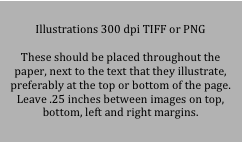
\includegraphics[width=3.31in]{figure.png}
% \caption{This is an example of figure caption. Note that all figures, and tables are to be referenced in the text. \copyright Respect Copyright.}
% \end{figure}

% \begin{figure*}
% 
\includegraphics[width=\textwidth]{two-column-figure.png}
% \caption{Example of a double-column figure with caption. \copyright Respect Copyright.}
% \end{figure*}

% Jason Hoelscher has argued that art, as a system of practice theory, is a complex adaptive system \citep[p.38]{HoelscherNtsOnAtctlytcAsthtcs2015}. It uses the concept of dynamic equilibrium to describe the balance between the drive for novelty and the gravitational pull of established patterns or “attractor basins” within this system \citep[pp.41-42]{HoelscherNtsOnAtctlytcAsthtcs2015}. This balance ensures that while art is perpetually evolving, it remains anchored within a broader discourse, allowing for the formation of information-entropic dissipative structures — artworks. These objects, rich in complexity and depth, invite continuous interpretation and re-interpretation, reflecting the co-evolutionary nature of artistic practice and theory as they adapt and respond to each other and to their changing contexts. 

% Hoelscher has also referred to art styles and to recurring motifs in art as attractors. For example:

% \begin{quote}
%     [...] the human figure constitutes an artistic attractor of great power and draw, being “an oscillatory limit cycle around which the system flows repeatedly” (Kauffman 1993, 176) \citep[pp.11-12]{HoelscherThPtcsOfPhsSpc2014}
% \end{quote}

% \begin{quote}
%     Art as we name and understand it in our societies — Art in the singular, with a capital A — was unknown to those who enjoyed themselves at the theatre, commissioned works from painters and sculptors, listened to religious concerts, or hired musicians for their feasts or ceremonies. This is not a merely lexical issue. Art did not exist as a common sphere of experience, not only because the practice of the arts was intended for different social purposes, but, above all, because these purposes were themselves part of a hierarchical division of human activities and of the human beings who engaged in them. \citep[p.25]{RanciereMdrnTms2022}
% \end{quote}

% The regime of representation is epitomised for Rancière by classical theatre, in which the two meanings of the word sense — sensing as in experiencing, and making sense as in to understand conceptually — are tightly coupled.

% \begin{quote}
%     The stage was thought of as a magnifying mirror where spectators could see the virtues and vices of their fellow human beings in fictional form. And that vision in turn was supposed to prompt specific changes in their minds: Molière’s Tartuffe supposedly taught spectators to recognize hypocrites; Voltaire’s Mahomet to fight for tolerance against fanaticism, and so on. Now, that ability to produce the dual effect of intellectual recognition and appropriate emotion was itself predicated on a regime of concordance inherent in representation.
% \end{quote}

% Art “as technics“, Sauvagnargues says, “concerns the way in which materials (matières) are captured and assembled into matter (matière) of expression.” \citep[p.75]{SauvagnarguesArtmchns2016}. However, art is not reducible to technics so that it does not require a specific kind of analysis \citep[p.74]{SauvagnarguesArtmchns2016}.


% Flack has referred to an earlier study in which she worked with a group of monkeys (pigtailed macaques) who used a silent, bared-teeth signal to communicate about their specific position in a power distribution, as if each individual monkey had a “power score”. The power score was a “course-grained representation of [...] an individual's fighting ability as collectively perceived by the group” \citep[p.5]{FlackCrsGrnng2017}. The power distribution was very stable\footnote{

%     During the study there was only one relationship reversal over the course of 5 months. \citep[p.1584]{FlackCntxtMdltsSgnlMnng2007}

% }. This silent bared-teeth signal was always used in interactions between only two monkeys and was only emitted by the monkey with a lower power score. Flack found that the signal occurred in two contexts:

% \begin{enumerate}
%     \item{
%         In response to aggression or threat of it
%     }
%     \item{
%         During pass-bys and approaches in the absence of any overt aggression or threatening behavior
%     }
% \end{enumerate}

% The first use case, when the signal was used during conflict, can be read in behaviourist terms as a simple stimulus response. In this case the signal functioned as an indicator of submission. Flack focused instead on the use of the signal during peaceful encounters and found that its use was always correlated with the position in the power distribution of each monkey. She has suggested that the signal, when used in this context “enabled communication about subordination, a pattern of behavior, rather than just submission in the present interaction” \citep[p.1584]{FlackCntxtMdltsSgnlMnng2007}.

% The pattern of power distribution within the social system of the monkeys was apparently functioning as a store of information about the relative capability of each monkey to win fights\footnote{

%     Presumably fighting ability correlates with some fitness parameters

% }. The signalling process was making the information available in an easy, low-energy (coarse-grained) form. There was no need for the monkeys to be constantly fighting in order to know where they are positioned, nor to remember the power distribution (to store it in their brain). A monkey only needed to maintain an awareness of their power score, which they gleaned from casual interactions and from watching the interactions of other monkeys\footnote{

%     The power score is not a number (of course) but an estimate of “the \emph{degree of consensus} in the group that they can win fights” \citep[p.5]{FlackCrsGrnng2017}.

% }. The stable power distribution, as it was continually reinforced through the network of interactions and signals, made possible otherwise costly conflict-management strategies, such as a kind of policing strategy in which the most powerful monkeys were unchallenged when they intervened to break up disputes \citep[p.5]{FlackCrsGrnng2017}.

% If Flack's distinction between \emph{coarse-graining in Nature} and \emph{coarse-graining by scientists} is valid, it would make the concept less useful. Addressing an imagined readership of scientists, Flack referred to ideas like temperature as “coarse-grainings that we as scientists impose on the system to find compact descriptions of system behaviour sufficient for good prediction.” In making a distinction between what scientists do and “how adaptive systems identify regularities and build effective theories to guide adaptive decision-making and behaviour”, Flack was apparently suggesting, or assuming, that communities of scientists working together to measure and observe phenomena are somehow not \emph{adaptive systems identifying regularities and building effective theories to guide adaptive decision-making and behavior}. Clearly they are, as Chang, Latour and Woolgar, and other philosophers and historians of science have shown\footnote{
    
%     See DeLanda's discussion of the way scientists produce theories, e.g. he quotes Alan Garfinkel (Forms of Explanation, pp. 53–8): “an object of explanation should be chosen which is stable under small perturbations of its conditions.” \citep[pp.161-162]{DeLandaIntnsvSci2013}

% }.

% Coarse-graining is a more useful concept if it is not divided into two different types, one for scientists and one for the rest of reality. Scientists are participants in a complex process that includes, depending on where one decides to draw the boundary, the full human and social context of particular scientists, science itself, various technologies, the phenomena under observation and even quantum entanglements. Flack's tendency to treat science as something separate from nature could perhaps be an example of course-graining. She has noted that components in a complex system can tune to a slow variable regardless of whether it actually does a good job of summarizing regularities. “Think”, she has advised us, ”of social institutions that are highly constraining and very hard to change” \citep[p.9]{FlackCrsGrnng2017}.

% In any case, those days are over.

% The American critic and philosopher of art Arthur Danto was one of the first to point out the absurdity of the idea that aesthetic experiences are synonymous with the experiences of beauty (and also that it is a kind of philosophical colonialism, since it requires a single subjective, culturally informed, experience to function as an objective definition \citep[p.124]{DantoEmbdMnngs2007}), and that a focus on beauty has had the effect of delegitimising the real diversity of aesthetic experiences artists routinely deploy \citep[p.59]{DantoThAbsOfBty2003}, which might be based in virtually any kind of observed quality, like cuteness \citep[p.28]{DantoThPhlsphclArt2005}, grunge, blandness \citep[p.126]{DantoEmbdMnngs2007}, disgustingness, eroticism, \citep[p.59]{DantoThAbsOfBty2003}, et cetera.

% A final example is Frank Stella's 1959 stripe paining \emph{The Marriage of Reason and Squalor II}. Which

% \begin{quote}
%     [...] appears to be as resolutely determinate and definite as a painting can be, a kind of no-nonsense record of the process of its own creation. The painting is simultaneously composed of, and comprises, two sets of twelve equally spaced and concentrically organized stripes, each of which is a flat uninflected brushstroke the width of the brush with which it was painted.
% \end{quote}

% Stella apparently described his goals for the painting in blunt terms as being to “keep the paint as good as it was in the can” \citep[p.38]{HoelscherArtAsInfrmtn2021}. He also said of it: “What you see is what you see” \citep[p.39]{HoelscherArtAsInfrmtn2021}. However, Hoelscher has suggested, the painting is not as simple as it appears.

% \begin{quote}
%     [...] By the time Stella painted his first stripe paintings in 1959, art's network of discursive entanglements had reached a state so charged with potential that it was able to produce artworks discursively coded as nondiscursive objects [...] each painting has been discursively coded as a simple and nondiscursive object, the simple nondiscursivity of which makes it discursively important according to a complex weave of artistic discourses built up over the course of a century.
% \end{quote}

% Hoelscher summed up the operation of Stella's painting in the same informational terms as the Morris sculpture and the Duchamp readymade.

% \begin{quote}
%     Enfolding multiple orders of operation that range from deadpan brushstrokes, to objecthood, to tautological statement, to large-scale discursive and cultural complexes of ideas, the Stella stripe painting + statement ensemble thus operates as a differential object, as a bundle of tightly entangled yet irresolvable differences that propagate still further difference.
% \end{quote}

% In the early 2000s, the mode of resonance between philosophical and scientific theories of complexity found conceptual form in the term \emph{complexity thinking}, which started to be used by scholars and practitioners working in fields like management theory, organisational change, health and education. At this time, Complex Adaptive Systems theory was filtering through into popular culture with memes like “chaos theory” and the concept of \emph{emergence} capturing the collective imagination. The term \emph{complexity thinking} expresses a sense of complexity as an intrinsic quality shared by diverse phenomena, and a sense of things being connected in unpredictable ways. The term acknowledges, according to Paul Cilliers and Kurt Richardson, the “...epistemological consequences of assuming the ubiquity of complexity” \citep{CilliersRichardsonCmplxtyScnc2001}. Complexity thinking describes an awareness that we can never fully know the dynamic interconnected processes at play within and between all phenomena. While it limits what we can reasonably claim to know, it also changes how we think about the world in ways that create new possibilities for knowing. 

% \begin{quote}
%     Having a basis in mechanism is a critical property of a coarse-grained description — it is “true” to the system. It is a simplification of the microscopic details. In principle, a coarse-grained description does not introduce any outside information to the subset of microscopic interactions over which it is performed [...] \citep[p.4]{FlackCrsGrnng2017}
% \end{quote}

% This paper examines how art might function, technically, by capturing our evolutionary capacity for aesthetic experience and deploying it to create meaning. The aim is to develop the idea of art as a technology so that it is available as a heuristic, a kind of effective theory\footnote{
%     An effective theory is one that is “able to organize phenomena under an efficient set of principles” and is also “not impossibly complex” \citep[p.1]{WellsEffctvThrs2012}. A good effective theory functions as a heuristic — a rule of thumb that can serve as a guide for action. The critical requirement is \emph{observational consistency} (an effective theory need not be even be true, as long as it works) \citep[p.71]{WellsEffctvThrs2012}.
% } that might open a space of possibility for us to have a different relationship with our technology.


    % Affect is one type of excess, or surplus product, of a system. Emergent properties are the result of the interaction of the components of a system, but they are not reducible to the properties of the components. All emergent properties of objects, including aesthetic properties, make objects more than the sum of their parts, as Aristotle said. It is the excess, or remainder, of the system that causes a qualitative shift (a phase-shift) in the system.

    % \begin{quote}
    %     If there were no escape, no excess or remainder, no fade-out to infinity, the universe would be without potential, pure entropy, death. Actually existing, structured things live in and through that which escapes them. Their autonomy is the autonomy of affect. \citep[pp.96-97]{MassumiTheAtnmyOfAffct1995}
    % \end{quote}

% Purpose is synonymous with Aristotle's concept of \emph{final cause}, and functions as an \emph{enabling constraint} \citep{JuarreroCsltyAsCnstrnt1998}, giving art objects meaning. Meaning\postnote{

%     DeLanda pointed out that the word \emph{meaning} is used in two different ways: to denote significance (as in “this life has a meaning”) and signification (as in “this word has a meaning”) \citep{DeLandaCsltyAndMnng2018}. Two forms of knowledge \citep[p.43]{DeLandaCsltyAndMnng2018} Meaning as signification is the most relevant in an art context, although both may apply.

% }, information (in the Simondonian sense), and aesthetic experience are all \emph{affect}. One person's embodied meaning \citep[p.125]{DantoEmbdMnngs2007}, is another's reorientational expansion and entanglement of aesthetic experience \citep[p.78]{HoelscherArtAsInfrmtn2021}.

% Kant's formulation that art is “...purposive without purpose...” \citep[p.57]{KantCrtqOfJdgmnt} is reformulated by complexity thinking, revealing art to be purposive with purposes that are `...indeterminate, expansive, many layered, and multidimensional...” \citep[p.25]{HoelscherThPtcsOfPhsSpc2014}. The purpose of an art object is always open, both to addition and to change. 


% Assemblage Theory enables us to recognise art, by its flexible boundaries and heterogeneous components, as an extremely deterritorialised assemblage. Art is a social system. The aesthetic regime is connected with all other social systems but maintains its identity — its autonomy — through codification. It is never possible to formalise the codes because they are always mutating. Boundaries in the aesthetic regime — say, between objects that are art and things that are not art — are extremely flexible. “Art exists as a separate world since anything whatsoever can belong to it” \citep[p.X]{RancièreAisthesis2013}. The system ot art consists of all art objects that have been and can be made, galleries, materials, artists, et cetera, as well as the diverse array of concepts, stories, and judgments that ascribe meaning to it. Wildly different objects created using diverse techniques for different purposes may be treated by the system as artworks. 

% While the knob of territorialisation in DeLanda's parametrised model of assemblages is turned way down for art, the knob of codification is turned way up. The aesthetic regime is a system of codes. Like the genetic codes that govern life, the codes that define what is and what isn't art at different times and in different contexts are not reducible to a set of rules. They are always in flux around concepts and beliefs which are themselves unstable. At any single moment, the system is characterised by a plurality of intersecting attitudes, agreements, disagreements and manifestos about art and aesthetic experience — including disagreement about whether art is about aesthetic experience. 

% Like all deterritorialised assemblages the art system is always in danger of capture — for example, by economic forces or by individuals.

% A style is an attractor state in the art assemblage. Art styles are technical subdomains, the results of bifurcations — symmetry breaking events within the system \citep[pp.165-170]{HalsallSystmsOfArt2008} \citep[pp.10-11,41-42]{HoelscherNtsOnAtctlytcAsthtcs2015}. A style is a virtual continuum, a set of potential forms that can be actualised in the production of art objects according to certain combinations of enabling constraints and purposes.

% Art evolves through complex combinatorial evolutionary processes. New styles are formed through the recombination of existing styles, the introduction of new materials and techniques, and the development of new purposes. The evolutionary processes of art are similar to those of biological evolution, including mutation, selection, exaptation, mutualisms, paedomorphosis and epigenesis. 

% Artists are active forces in the evolutionary processes of art, the creation and maintenance of the codes that define what art is and what it can do. Referring to the painter Barnett Newman's famous quip “Aesthetics is for me like ornithology must be for the birds” \citep[p.253]{MattickAsthtcsAndAntAsthtcsInThVslArts1993}, Paul Mattick noted that ”...artists, unlike birds in the wild, are engaged in a cultural and therefore historically evolving activity. For this reason aesthetics is actually quite unlike ornithology. The birds do not, for example, question the concepts evolved by theorists to describe their activities” \citep[p.258]{MattickAsthtcsAndAntAsthtcsInThVslArts1993}.

% \section{Contemporary Technology-based Art}\label{sec:ContemporaryTechnologyBasedArt}

%     If we consider that the world is full of potential information, that the disorder of the world is “...a highly charged and catalytic mode of entropy akin to information entropy — not inert, but saturated to bursting with potentials that are oriented toward actualization.” \citep[p.72]{HoelscherArtAsInfrmtn2021}, then Contemporary art is a way of actualising certain information, of making certain relations visible. These relations may be fictional, speculative, false or even impossible. Art can actualise new potential realities, new ways of being, new ways of seeing. Or it can make visible the hidden relations of the world as it is.

%     Art that utilises emerging technologies is, unavoidably, Contemporary. The purposes of technology-based art includes making visible the hidden relations of technological systems, and calling into being new socio-technological realities.